\documentclass[a4paper,12pt,abstracton]{scrartcl}
\usepackage[utf8]{inputenc}
\usepackage{float}
\usepackage{tikz}
\usepackage{amsmath}
\usepackage{amssymb}
\usepackage{pifont}% http://ctan.org/pkg/pifont
\usepackage[font=small,labelfont=bf]{caption}
\usepackage{graphicx}
\usepackage{dirtytalk}
\usepackage{multicol}
\usepackage{booktabs}
\usepackage{colortbl}
\usepackage{appendix}
\usepackage{nomencl}
\usepackage{lmodern}
\usepackage[nottoc]{tocbibind}
\usepackage{xcolor}
%\graphicspath{images/}
\usepackage[margin = 3cm]{geometry}
\usepackage{ragged2e} % good alignment
\usepackage{hyperref}
\usepackage{siunitx} % Provides the \SI{}{} and \si{} command for typesetting SI units
\hypersetup{colorlinks=true,
    linkcolor=blue,
    filecolor=magenta,      
    urlcolor=cyan, 
    citecolor=gray}

%\DeclareGraphicsExtensions{.png,.pdf} % low-res (work in progress)
%\DeclareGraphicsExtensions{.pdf,.png}  % high-res (final draft)
%\setlength\parindent{0pt} % Removes all indentation from paragraphs
%\bibliographystyle{unstr}
\setlength\parindent{0pt}
\setlength{\parskip}{0.3em}
\newcommand{\xmark}{\ding{55}}

\renewcommand{\nomname}{List of Symbols}
\renewcommand{\nompreamble}{The following list explains the symbols used within the body of the report.}

\usepackage{etoolbox}
\renewcommand\nomgroup[1]{%
  \item[\bfseries
  \ifstrequal{#1}{E}{Experimental Equipment}{%
  \ifstrequal{#1}{C}{Computational Methods}{%
  \ifstrequal{#1}{T}{Theoretical Concepts}{
  \ifstrequal{#1}{P}{Physical Constants}{}}}}%
]}


\subject{CMP Lab Report} % Matter Physics, Physics, Chemical Physics ?
\title{Zeeman Effect}
\author{Group B9\footnote{Pietro Monticone , Claudio Moroni , Alberto Mosso , Riccardo Valperga.}}

\renewcommand{\listfigurename}{Plots}
\renewcommand{\listtablename}{Tables}
\renewcommand{\nomname}{Nomenclature}


\begin{document}
\maketitle
\makenomenclature
\begin{abstract}
This experiment examined the normal and anomalous Zeeman effect with the aim of calculating the Bohr magneton by fitting the energy gap between spectral lines of a cadmium lamp immersed in a magnetic field, as a function of its magnitude. The first section concerns the magnet calibration and the procedure we adopted to test the magnetic field homogeneity. As far as the former is concerned, we expected the magnetic field to vary almost linearly with the current since we worked with soft ferromagnets. Regarding the latter, we have made sure that for small displacements in the region occupied by the cadmium lamp, the magnitude of the magnetic field did not vary substantially. Lastly, after the global experimental apparatus has been endowed with polarizing filters, a CCD camera and a retarding lamina, several images of the splitted spectral lines have been taken in various states depending from the chosen orientation (longitudinal or traversal) of the magnets with respect to the optical axe and the configuration of the polarizing filters placed along the light path. The results consist of four estimates of the Bohr magneton and the relevant compatibility tests .
\end{abstract}
\clearpage
\tableofcontents
%\listoffigures
%\listoftables

\mbox{
\nomenclature[E]{CCD}{Charge-Coupled Device}
\nomenclature[P]{$m_e$}{Electronic Mass}
\nomenclature[P]{$e$}{Electronic Charge}
\nomenclature[P]{$\mu_B$}{Bohr Magneton}
\nomenclature[P]{$h$}{Plack Constant}



\nomenclature[T]{$\vec{B}$}{Magnetic Field}
\nomenclature[T]{${B}=|\vec{B}|$}{Magnetic Field Magnitude}
\nomenclature[T]{$I$}{Electric Current}
\nomenclature[T]{$\mu_{X\in\{N,A\}}^{Y\in\{T,L\}}$}{Magnetic Moment in $(X,Y)$}
\nomenclature[T]{$g$}{Gyromagnetic Factor}
\nomenclature[T]{$g_{q\in\{n,a\}}$}{\say{Normal}/\say{Anomalous} Gyromagnetic Factor}
} % FINIRE MERDE!!!
\clearpage
\setlength{\columnsep}{27pt} 
\begin{multicols}{2}
\printnomenclature
\end{multicols}
\newpage

\section{Theoretical Introduction}\label{sec: ThIntro}
Zeemann effect is a phenomenon where the submission of a spectroscopic light source to a magnetic fields causes the splitting of the observed spectral lines. Because a spectral line is associated to an atomic energy level, such splitting is always related to a degeneracy breaking. In an atom, degeneracy is due to the orbital momentum l, its third component $m_l$, and the z-component of spin $m_s$ (s is fixed  because electrons are fermions, so $s=\frac{1}{2}$.\newline
Normal Zeemann effect is observed when the total spins of the base and target level of the transition are zero.
Anomalous Zeeman effect is instead detected when the spins of the base and target level of the transition are not zero.
\subsection{Normal Zeemann effect}
An external magnetic field $\vec{B}$ gives an energy contribution to each level
\begin{equation}
\Delta E = - \vec{\mu} \cdot \vec{B}
\end{equation}
Where $\vec{\mu}$ is the magnetic moment. We consider $\vec{B}$ parallel to the z-axis, so we are only interested in $\mu_z$. One finds: 
\begin{equation}
mu_z \equiv -\frac{e}{2m}L_z = -\frac{e}{2m}\hbar m_lg_l
\end{equation}
Where $g_l$ is a constant equal to 1.Thus:
\begin{equation}
\Delta E = - \mu_z B = \frac{e \hbar}{2m} m_l B = \mu_B m_l B
\end{equation}
Where $\mu_B$ is the Bohr's magneton, whose theoretical value is
$\mu_B = $. Because $\Delta E$ depends on $m_l$, degeneracy in $m_l$ is broken and thus spectral lines split.
\subsection{Anomalous Zeemann Effect}
When spin is involved, the expression for $\vec{\mu}$ to use is 
\begin{equation}
\vec{\mu}=-\frac{eg_l}{2m} \vec{L}_J - \frac{eg_s}{2m} \vec{S}_J
\end{equation}
Where $\vec{L}_J$ and $ \vec{S}_J$ are the projections of $\vec{L}$ and $\vec{S}$ along the total angular momentum $\vec{J}:= \vec{L}+ \vec{S}$, and $g_s$ is about 2. One finds:
\begin{equation}
\vec{\mu} = -\frac{e}{2m}g_{jls}\vec{J}
\end{equation}
Where 
\begin{equation}
g_{jls}=\frac{3j(j+1)-l(l+1)+s(s+1)}{2j(j+1)}
\end{equation}
Pointing $\vec{B}$ along the z-axis, we have $\mu_z =-\frac{e \hbar}{2m}g_{jls}m_j=-\mu_B g_{jls}m_j$, thus
\begin{equation}
\Delta E = -\vec{\mu}\cdot \vec{B}= \mu_z B = \mu_Bg_{jls}m_j B
\end{equation}
When considering anomalous Zeemann effect, both spinorial and orbital degeneracy are broken, giving rise to even more splitting.
\clearpage
\section{Experimental Introduction}\label{ExpIntro}
\subsection{Calibration \& Magnetic Field Homogeneity Test}
\subsubsection{Apparatus}
The apparatus is composed of two ferromagnetic-core electromagnetic expansions connected to a current generator, an amperometer ***insert amperometer type NO*** and a magnetometer ***insert magnetomenter name NO***.
\subsubsection{Procedure}
The first goal is to extrapolate from a series of measurements a B(I) relation, where B is the magnetic field and I the current flowing through the expansions. 
Using the following circuit \footnote{The capacity C is large and it is there for safety reasons, should one accidentally induce a short-circuit.}
\begin{figure}[H]
\begin{center}
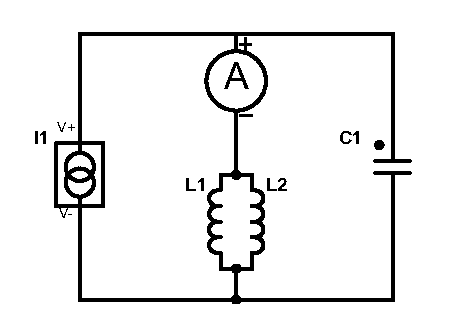
\includegraphics[trim=0cm 0cm 0cm 0cm,clip,width=7.5cm,keepaspectratio]{images/circuito.pdf} 
\caption{circuital scheme used}
\end{center} 
\end{figure}
The current has been varied about 1A stepwise (read on the amperometer) and the magnetic field measured in the middle of the expansions. The current sequences $0A \longrightarrow 10A \longrightarrow 0A \longrightarrow 10A$ were performed.
Then, by choosing a specific current value, the magnetic field has been measured at different positions between the expansions. This was needed on order to assign a more precise uncertainty to the values of B.
\subsection{Zeeman Effects}
\subsubsection{Apparatus}
An optical bench endowed with a cadmium spectroscopic light source inserted between the electromagnets discussed above, a diaphragm, a Fabry-Perot interferometer, a wavelength filter, a polarizer, a retarding lamina and A CCD camera has been used. A particular wavelength $\lambda$ interval of the light coming from the source was selected via the filter before entering the interferometer. Because of the functioning of the Fabry-Perot interferometer an input wavelength is diffracted in a series of circular spectral lines. As the filter acts on an interval of $\lambda$,we could observe the splitting of a wavelength into two/three (normal logitudinal/transverse effect : see \ref{subsec:1}) or six/nine (longitudinal/transverse anomalous), without dealing with extra lines. The Fabry-Perot interferometer main characteristic is the following:\newline
defined $$\delta = r^2_{n,a}-r^2_{n,b}$$ and $$\Delta = r^2_{n+1,a}-r^2_{n,a}$$  where $r_{n,a}$ is the radius of the n-th order spectral line corresponding to the wavelength a, we have that $\delta$ and $\Delta$ are approximately constant with respect to n and $\lambda$ when $a\simeq b$. Moreover, by geometric means, one finds that 
\begin{equation} \label{eq:1}
\Delta E  = \frac{hc}{2\mu t} \frac{\delta}{\Delta}
\end{equation}
 where $\mu$ is the refracive index of the interferometer and t is its thickness. So one is able to calculate $\Delta E$ from the images acquired form the CCD camera.
\subsubsection{Procedure} \label{subsec:1}
The experimental procedures followed to observe the normal zeemann effect and the anomalous one were similar. The magnets could be rotated, giving rise to the possibility of perpendicular and longitudinal configurations (orientations are referred to the optical bench axis). When considering the former, output light was linearly polarized (one could choose to observe the 2 linear polarizations by rotating the axis of the polarizer, no retarding lamina needed); the latter returned circularly polarized light: the lamina was used in combinations with the polarizer. It is to be said that in longitudinal configuration a light component, namely the one that would have polarization parallel to propagation direction, disappeared.\newline
Wavelength $643.847 nm$ corresponding to $3 ^{1}D_{2} \longrightarrow 2 ^{1}P_{1}$  transition was selected to observe normal zeeman effect, while wavelength $508.588 nm$ corresponding to $3 ^3S_1 \longrightarrow 2 ^3P_2$ was chosen to observe the anomalous one. \newline
At each value of the current flowing through the electromagnets three snapshots (diffractograms) of the CCD were taken: the first depicting all lines, the second and the third were retrieved after inserting the polarizer and selecting one polarization and the other. This was executed for both the normal and anomalous settings, in transverse and longitudinal configurations.\newline
Thus for each value of current (i.e. for each value of magnetic field extrapolated from the B-I curve one got before) we had many values of $\delta \text{ and } \Delta $ (all we could get form the three CCD snapshots), whose averages were to be used to get $\Delta E$ from \ref{eq:1}. Measures of $\delta$ and $\Delta$ were taken on diffractograms using Motic Images Plus 3.0 software.
Thus one ends up with four linear fits of $\Delta E \text{ vs } B$, from which we could get four estimates of $\mu_B$, that were then compared, averaged and compared with the theoretical value. According to $g_{jls} , \; m_l \text{ and } m_j$ values, we used $\Delta E = \mu_B B$ to fit normal zeemann effect data, and $\Delta E =\frac{1}{2} \mu_B B$ for the anomalous one.
\clearpage
\section{Calibration}\label{sec:cal}

\subsection{Data Collection}
In order to calibrate the magnet it is necessary to establish the dependence of the magnetic field $B$ from the current $I$ injected in the coils. Therefore we gradually increased and then decreased $I$ as shown in \hyperref[table:BI1]{Table \ref*{table:BI1}}  and \hyperref[table:BI2]{ \ref*{table:BI2}} respectively. 

\begin{table}[H]
\centering
\caption{}
\label{table:BI1}
\begin{tabular}{c c}
\addlinespace
\addlinespace
\resizebox{6cm}{!}{
\begin{tabular}{cc}
\toprule
$I\;[A]$ & $B\;[T]$\\
\midrule
 0.00 $\pm$ 0.02 & 0.000 $\pm$ 0.001\\
 1.02 $\pm$ 0.02 & 0.071 $\pm$ 0.001\\
  2.03 $\pm$ 0.02 & 0.140 $\pm$ 0.001\\
 3.00 $\pm$ 0.02 & 0.205 $\pm$ 0.001\\
  4.04 $\pm$ 0.02 & 0.277 $\pm$ 0.001\\
4.99 $\pm$ 0.02 & 0.342 $\pm$ 0.001\\
  6.02 $\pm$ 0.02 & 0.408 $\pm$ 0.001\\
7.00 $\pm$ 0.02 & 0.471 $\pm$ 0.001\\
  8.02 $\pm$ 0.02 & 0.535 $\pm$ 0.001\\
8.48 $\pm$ 0.02 & 0.563 $\pm$ 0.001\\
 9.01 $\pm$ 0.02 & 0.588 $\pm$ 0.001\\
9.51 $\pm$ 0.02 & 0.612 $\pm$ 0.001\\
 10.04 $\pm$ 0.02 & 0.636 $\pm$ 0.001\\
\bottomrule
\end{tabular}}
\hspace{2cm}
\resizebox{6cm}{!}{
\begin{tabular}{cc}
\toprule
$I\;[A]$ & $B\;[T]$\\
\midrule
  10.04 $\pm$ 0.02 & 0.636 $\pm$ 0.001\\
 9.50 $\pm$ 0.02 & 0.613 $\pm$ 0.001\\
8.97 $\pm$ 0.02 & 0.590 $\pm$ 0.001\\
 8.49 $\pm$ 0.02 & 0.566 $\pm$ 0.001\\
7.00 $\pm$ 0.02 & 0.478 $\pm$ 0.001\\
  6.05 $\pm$ 0.02 & 0.416 $\pm$ 0.001\\
4.98 $\pm$ 0.02 & 0.348 $\pm$ 0.001\\
 4.02 $\pm$ 0.02 & 0.282 $\pm$ 0.001\\
3.00 $\pm$ 0.02 & 0.215 $\pm$ 0.001\\
 2.00 $\pm$ 0.02 & 0.145 $\pm$ 0.001\\
1.00 $\pm$ 0.02 & 0.078 $\pm$ 0.001\\
 0.00 $\pm$ 0.02 & 0.009 $\pm$ 0.001\\
\\
\bottomrule
\end{tabular}}
\end{tabular}
\end{table}
\begin{table}[H]
\centering
\caption{}
\label{table:BI2}
\begin{tabular}{c c}
\addlinespace
\addlinespace
\resizebox{6cm}{!}{
\begin{tabular}{cc}
\toprule
$I\;[A]$ & $B\;[T]$\\
\midrule
 0.00 $\pm$ 0.02 & 0.009 $\pm$ 0.001\\
  0.99 $\pm$ 0.02 & 0.072 $\pm$ 0.001\\
1.97 $\pm$ 0.02 & 0.138 $\pm$ 0.001\\
  3.03 $\pm$ 0.02 & 0.208 $\pm$ 0.001\\
4.02 $\pm$ 0.02 & 0.276 $\pm$ 0.001\\
  5.04 $\pm$ 0.02 & 0.345 $\pm$ 0.001\\
6.00 $\pm$ 0.02 & 0.409 $\pm$ 0.001\\
  7.02 $\pm$ 0.02 & 0.475 $\pm$ 0.001\\
8.06 $\pm$ 0.02 & 0.540 $\pm$ 0.001\\
  8.46 $\pm$ 0.02 & 0.561 $\pm$ 0.001\\
9.02 $\pm$ 0.02 & 0.590 $\pm$ 0.001\\
 9.57 $\pm$ 0.02 & 0.616 $\pm$ 0.001\\
10.06 $\pm$ 0.02 & 0.637 $\pm$ 0.001\\
\bottomrule
\end{tabular}}
\hspace{2cm}
\resizebox{6cm}{!}{
\begin{tabular}{cc}
\toprule
$I\;[A]$ & $B\;[T]$\\
\midrule
10.06 $\pm$ 0.02 & 0.637 $\pm$ 0.001\\
 9.50 $\pm$ 0.02 & 0.613 $\pm$ 0.001\\
8.97 $\pm$ 0.02 & 0.590 $\pm$ 0.001\\
  8.49 $\pm$ 0.02 & 0.566 $\pm$ 0.001\\
7.00 $\pm$ 0.02 & 0.478 $\pm$ 0.001\\
  6.05 $\pm$ 0.02 & 0.416 $\pm$ 0.001\\
4.98 $\pm$ 0.02 & 0.348 $\pm$ 0.001\\
  4.02 $\pm$ 0.02 & 0.282 $\pm$ 0.001\\
3.00 $\pm$ 0.02 & 0.215 $\pm$ 0.001\\
  2.00 $\pm$ 0.02 & 0.145 $\pm$ 0.001\\
1.00 $\pm$ 0.02 & 0.078 $\pm$ 0.001\\
  0.00 $\pm$ 0.02 & 0.009 $\pm$ 0.001\\
  \\
\bottomrule
\end{tabular}}
\end{tabular}
\end{table}
\subsection{Data Analysis \& Visualization}
For sufficiently high values of $I$ the magnet exhibits a non-linear response which constrains us to fit the datasets with both linear and parabolic models in different domains as shown in \hyperref[fig:BI1]{Figure \ref*{fig:BI1}}  and \hyperref[fig:BI2]{ \ref*{fig:BI2}} .
$$
\begin{cases}
f(I)=\boldsymbol{a} I + \boldsymbol{b} \quad \forall I \leq 7.00 \pm 0.02 \text{ A} \\ \\
g(I)= \boldsymbol{a_p}I^2 + \boldsymbol{b_p}I + \boldsymbol{c_p} \quad \forall I > 7.00 \pm 0.02 \text{ A}
\end{cases}
\;\;
\begin{cases}
f(I)=\boldsymbol{p_0} I + \boldsymbol{p_1} \quad \forall I \leq 7.00 \pm 0.02 \text{ A} \\ \\
g(I)= \boldsymbol{a_p}I^2 + \boldsymbol{b_p}I + \boldsymbol{c_p} \quad \forall I > 7.00 \pm 0.02 \text{ A}
\end{cases}
$$
\begin{figure}[H]\hspace{-0.8cm}
    \begin{tabular}{c c}
      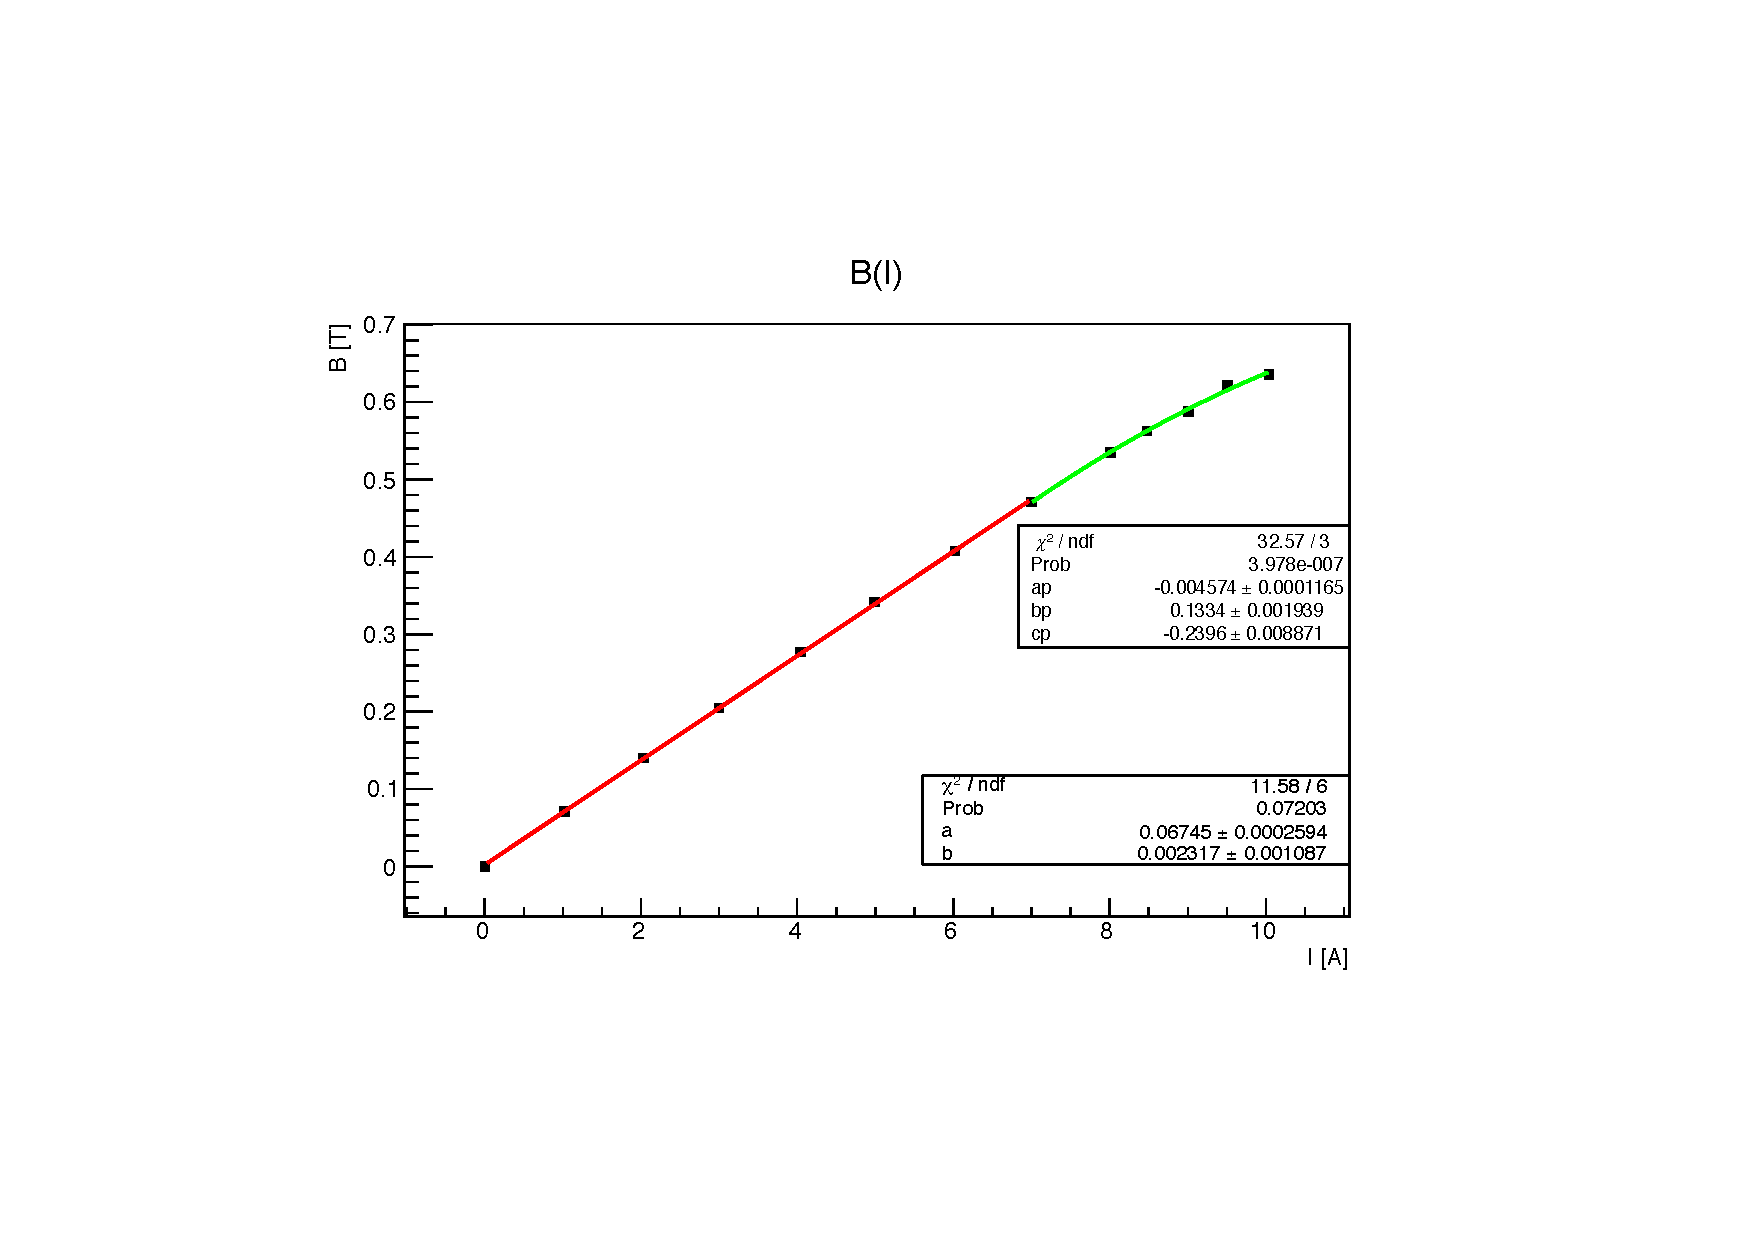
\includegraphics[scale=0.46]{plots/BIcre1.pdf}  &\hspace{0.1cm} 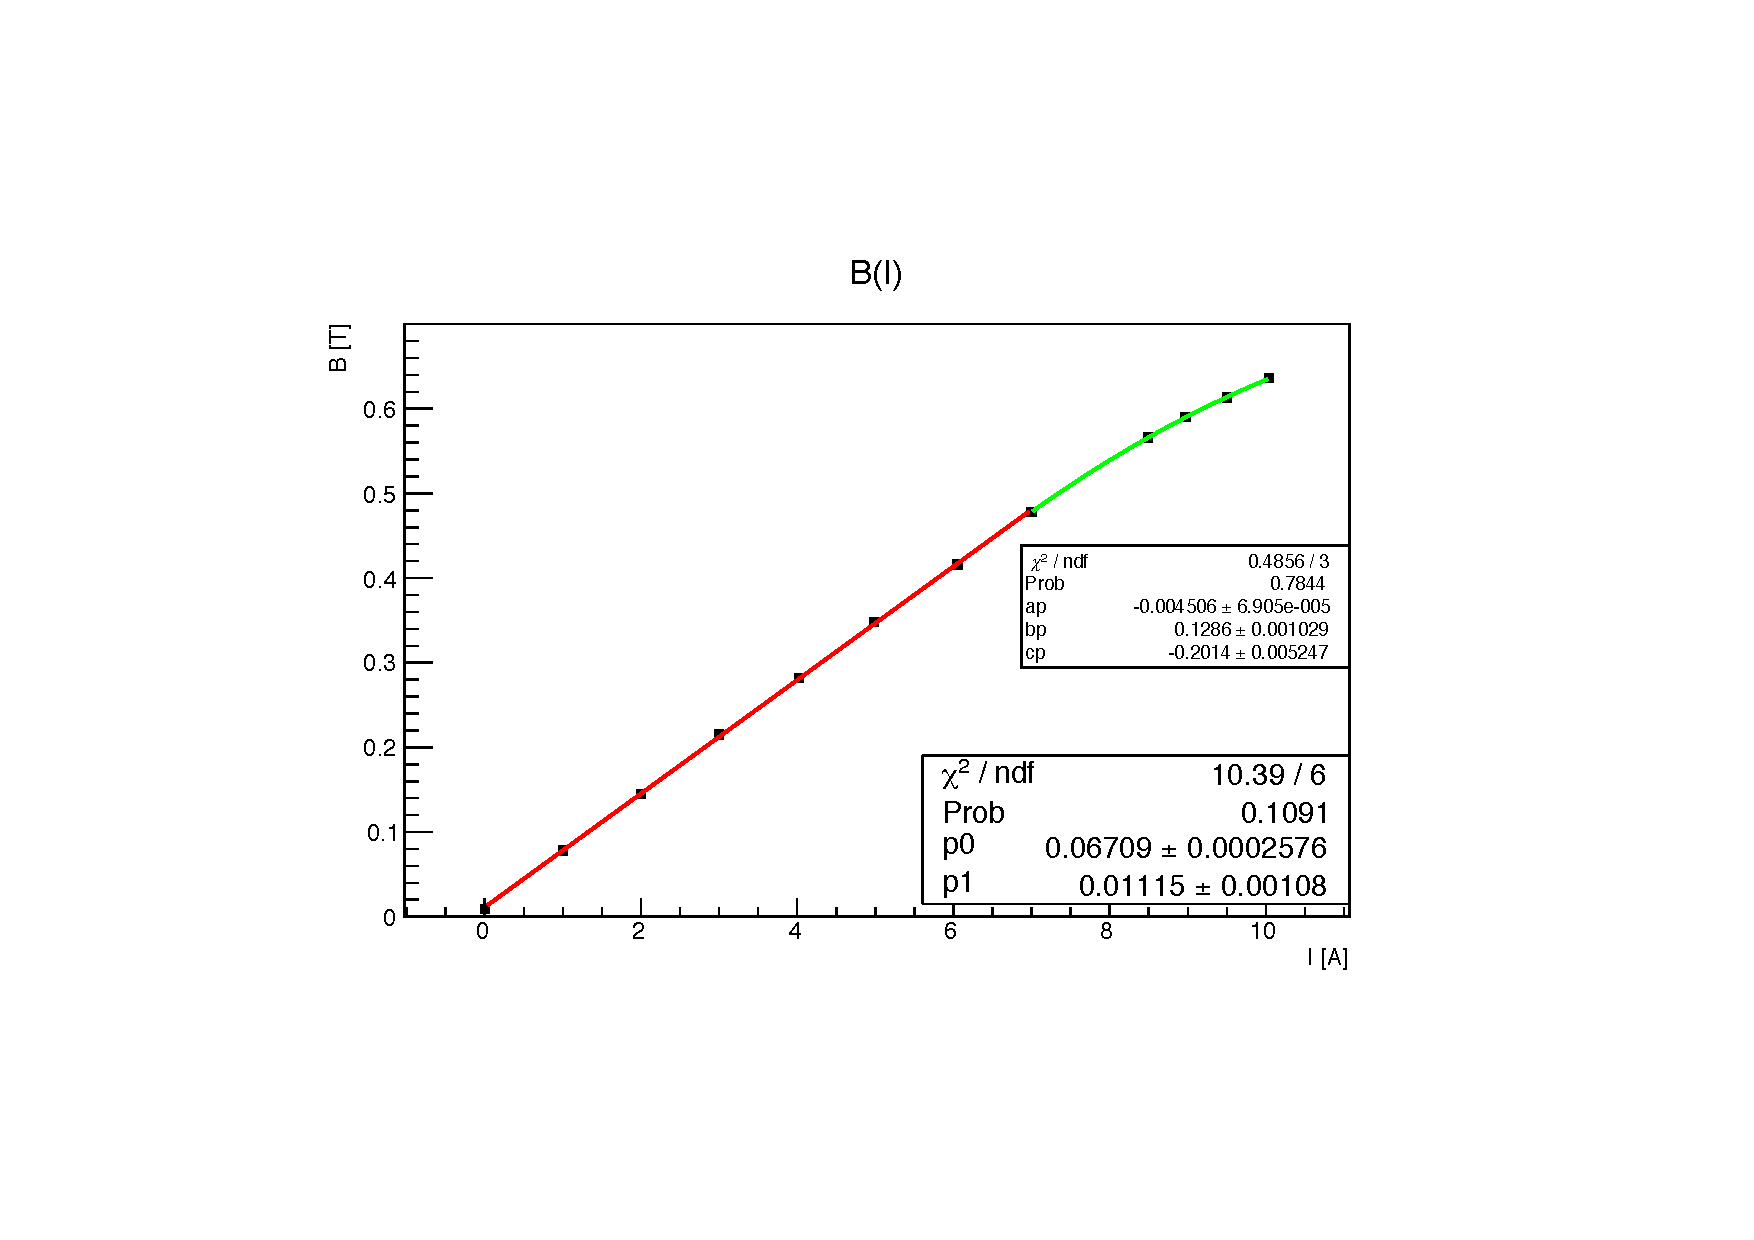
\includegraphics[scale=0.46]{plots/BIdec1.pdf} \\
      \end{tabular}
    \caption{}
    \label{fig:BI1}
\end{figure}
$$
\begin{cases}
f(I)=\boldsymbol{a} I + \boldsymbol{b} \quad \forall I \leq 7.02 \pm 0.02 \text{ A} \\ \\
g(I)= \boldsymbol{a_p}I^2 + \boldsymbol{b_p}I + \boldsymbol{c_p} \quad \forall I > 7.02 \pm 0.02 \text{ A}
\end{cases}
\;\;
\begin{cases}
f(I)=\boldsymbol{p_0} I + \boldsymbol{p_1} \quad \forall I \leq 7.00 \pm 0.02 \text{ A} \\ \\
g(I)= \boldsymbol{a_p}I^2 + \boldsymbol{b_p}I + \boldsymbol{c_p} \quad \forall I > 7.00 \pm 0.02 \text{ A}
\end{cases}
$$

\begin{figure}[H] \hspace{-0.8cm}
    \begin{tabular}{c c}
      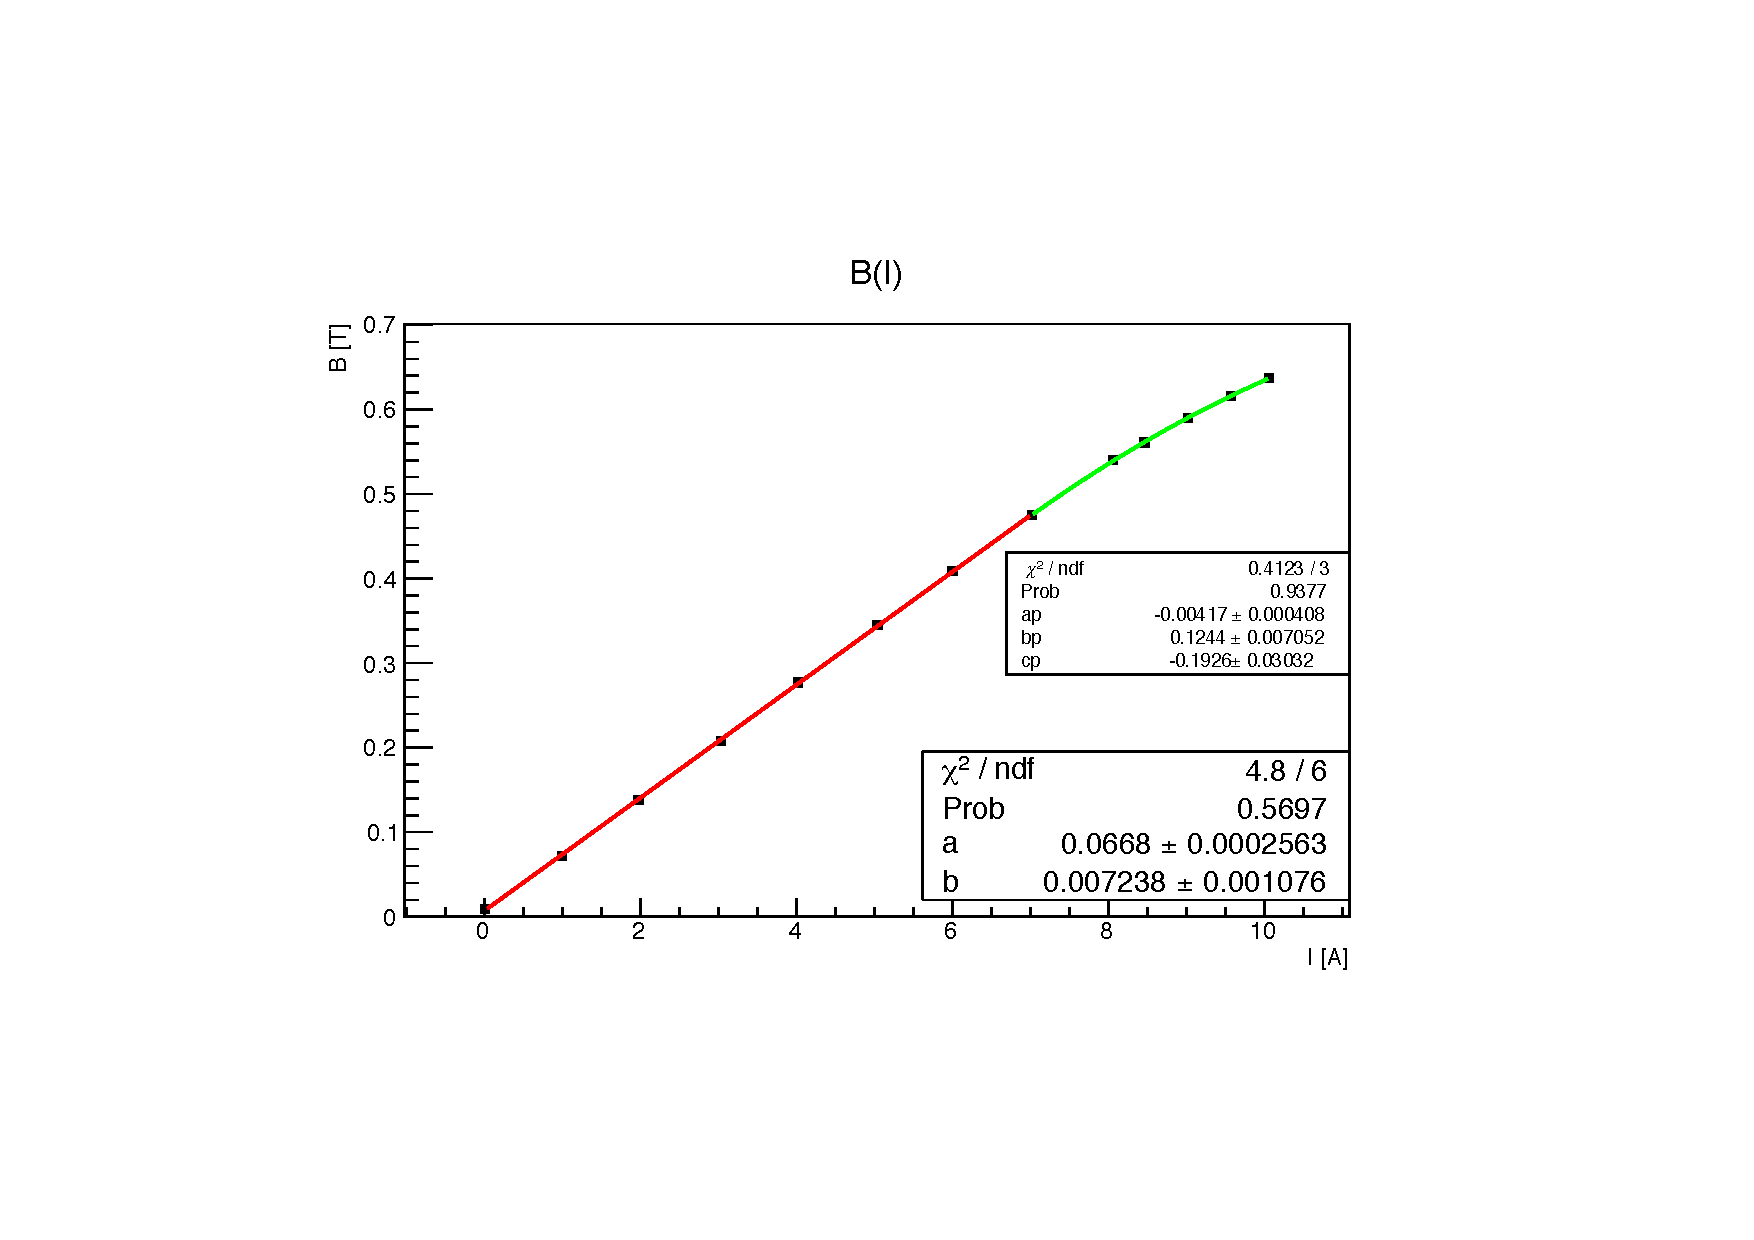
\includegraphics[scale=0.46]{plots/BIcre2.pdf}  &\hspace{0.1cm} 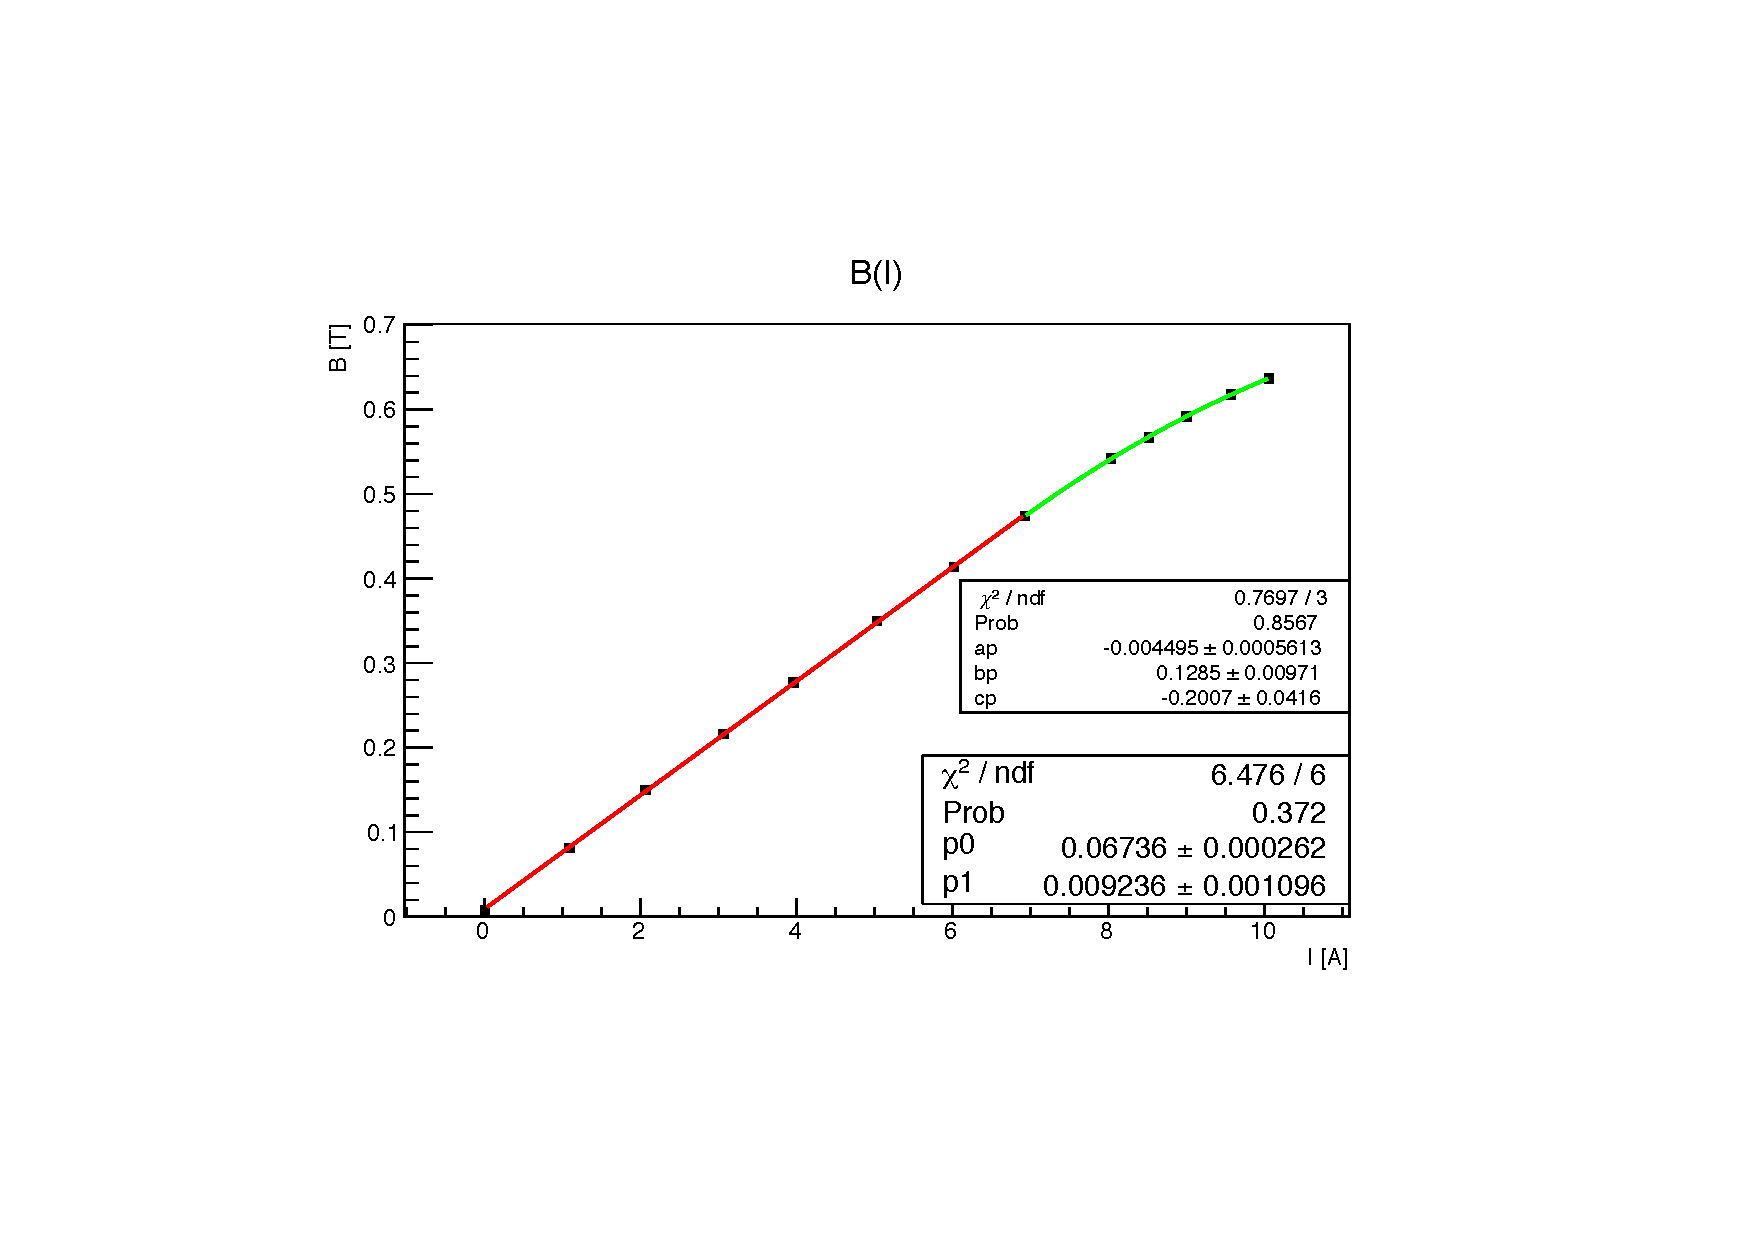
\includegraphics[scale=0.46]{plots/BIdec2.pdf} \\
      \end{tabular}
    \caption{}
    \label{fig:BI2}
\end{figure}
\clearpage
The final calibration curve reported in \hyperref[fig:calcurve]{Figure \ref*{fig:calcurve}} has been calculated as follows: 
\begin{enumerate}
    \item the four values of each parameter have been averaged ;
    \item the compatibility test between every single one with the global average has been computed ;
    \item the compatible ones has been used to get the final curve and their average has been shown to be compatible with the global one.
\end{enumerate}

It might be interesting to observe that, although the magnet we have worked with was a soft ferromagnet, the final calibration curve exhibits a residual magnetization measuring approximately 7 mT . 

\begin{figure}[H]
    \centering
    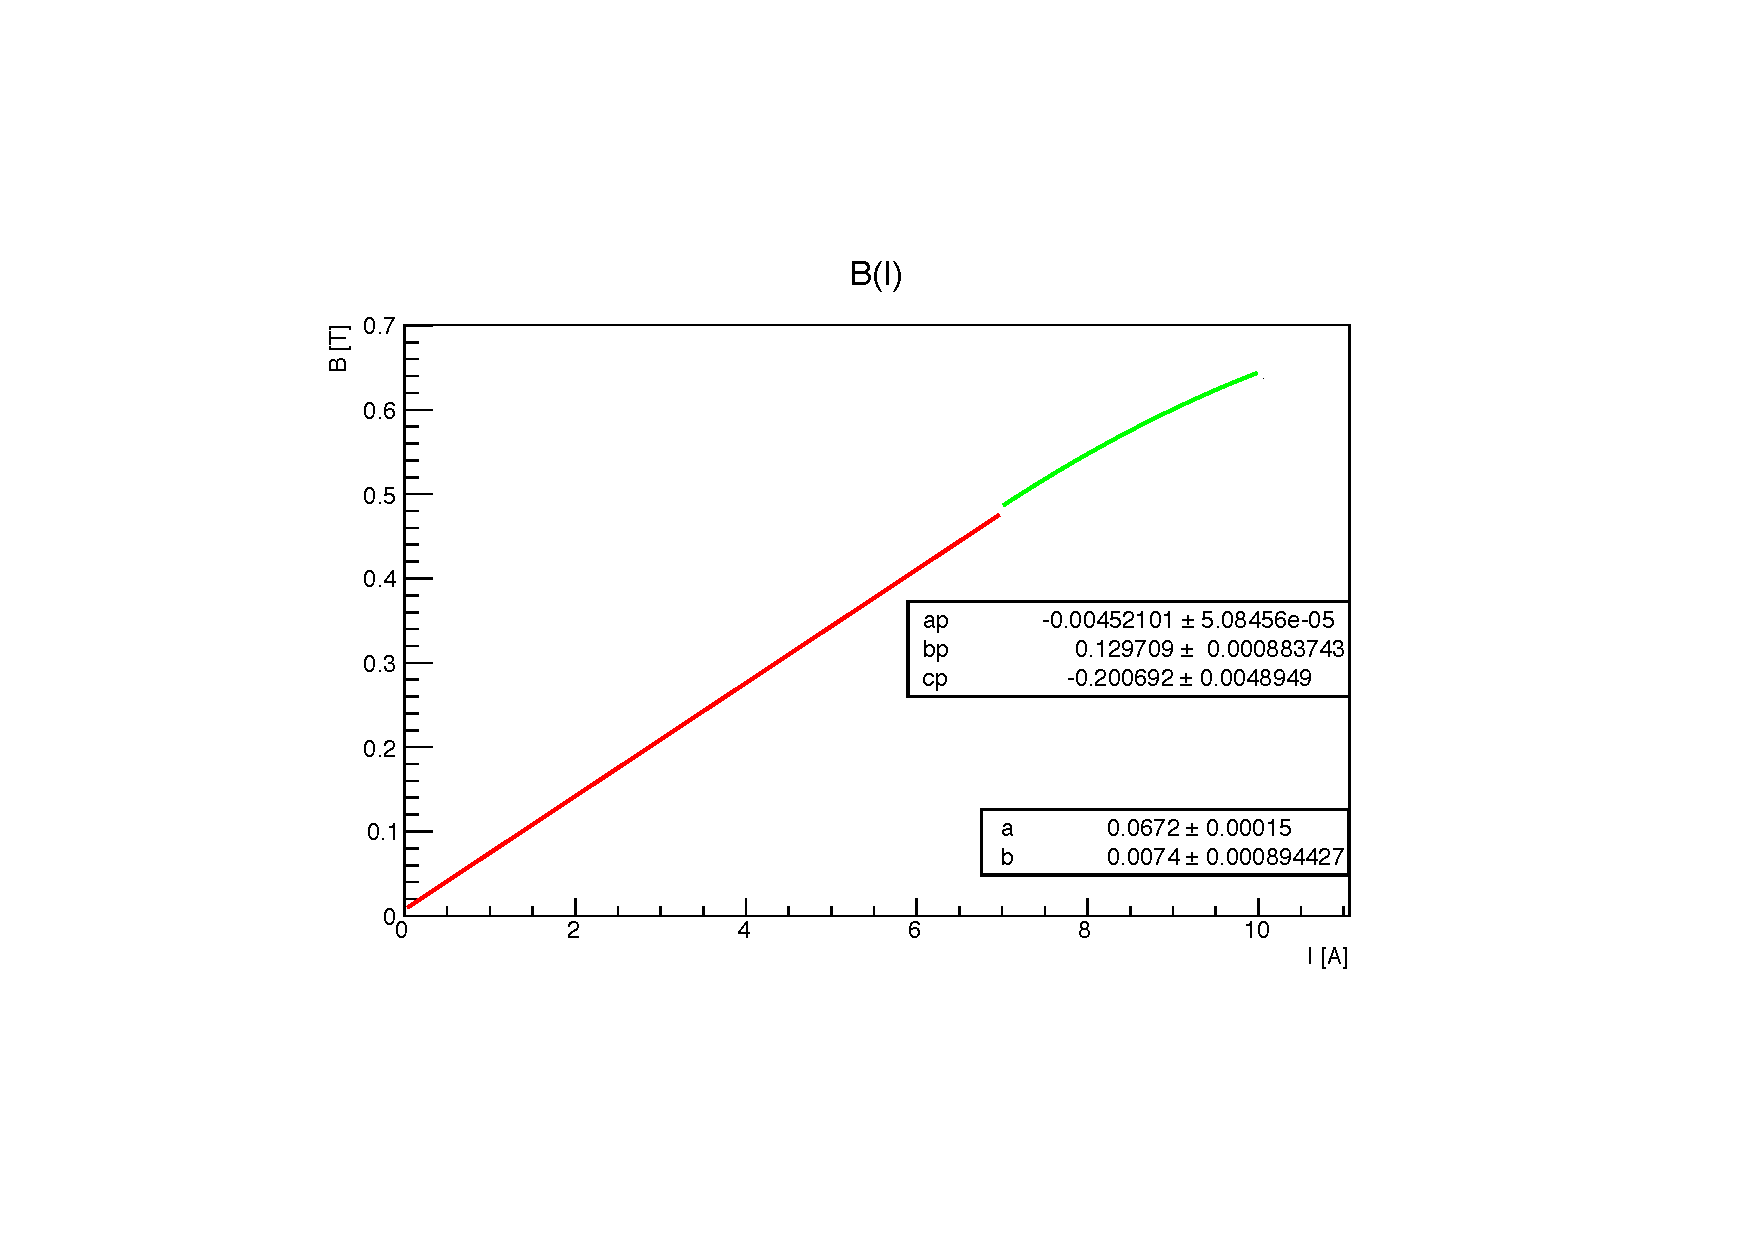
\includegraphics[scale=0.8]{plots/curva.pdf}
    \caption{}
    \label{fig:calcurve}
\end{figure}
From now on the compatibility tests will be evaluated according to the following rules and will never be explicitly stated again in the entire work: 

$$\begin{cases}
Z=\frac{|y-x|}{\sqrt{\delta y^2+ \delta x^2}} \\\\
Z_c = 1.96 \quad(\alpha=0.05) \\\\
\text{Compatibility condition:}\quad Z < Z_c
\end{cases}
$$

\clearpage
\section{Magnetic Field Homogeneity Test}
As anticipated in the \hyperref[sec:Intro]{Introduction}, in order to assign a proper uncertainty to the magnitude of the magnetic field $B$, it is necessary to evaluate its uniformity between the expansions. Therefore we took five measures of $B$ along a chosen horizontal diameter $x$, which have been reported in \hyperref[table:disX]{Table \ref*{table:disX}} and other five along the vertical $y$ reported in \hyperref[table:disY]{Table \ref*{table:disY}}. The relevant scatterplots have been displayed in \hyperref[fig:disX]{Figure \ref*{fig:disX}} and \hyperref[fig:disY]{ \ref*{fig:disY}} respectively.

\begin{table}[H]
\centering
\caption{}
\label{table:disX}
\resizebox{11cm}{!}{
\begin{tabular}{ccc}
\toprule
$I\;[A]$ & $x$ [mm] & $B\;[T]$       \\
\midrule
\rowcolor{gray!6}  4.20 $\pm$ 0.02 & -10.23 $\pm$ 0.05 & 0.248 $\pm$ 0.001 \\
 & -7.10 $\pm$ 0.05 & 0.278 $\pm$ 0.001 \\
\rowcolor{gray!6}   & -4.15 $\pm$ 0.05 & 0.285 $\pm$ 0.001 \\
 & 0.00 $\pm$ 0.05 & 0.285 $\pm$ 0.001 \\
\rowcolor{gray!6}   & 4.15 $\pm$ 0.05 & 0.285 $\pm$ 0.001 \\
 & 7.10 $\pm$ 0.05 & 0.278 $\pm$ 0.001 \\
\rowcolor{gray!6}   & 10.23 $\pm$ 0.05 & 0.247 $\pm$ 0.001 \\
\bottomrule
\end{tabular}}
\end{table}

\begin{figure}[H]
\begin{center}
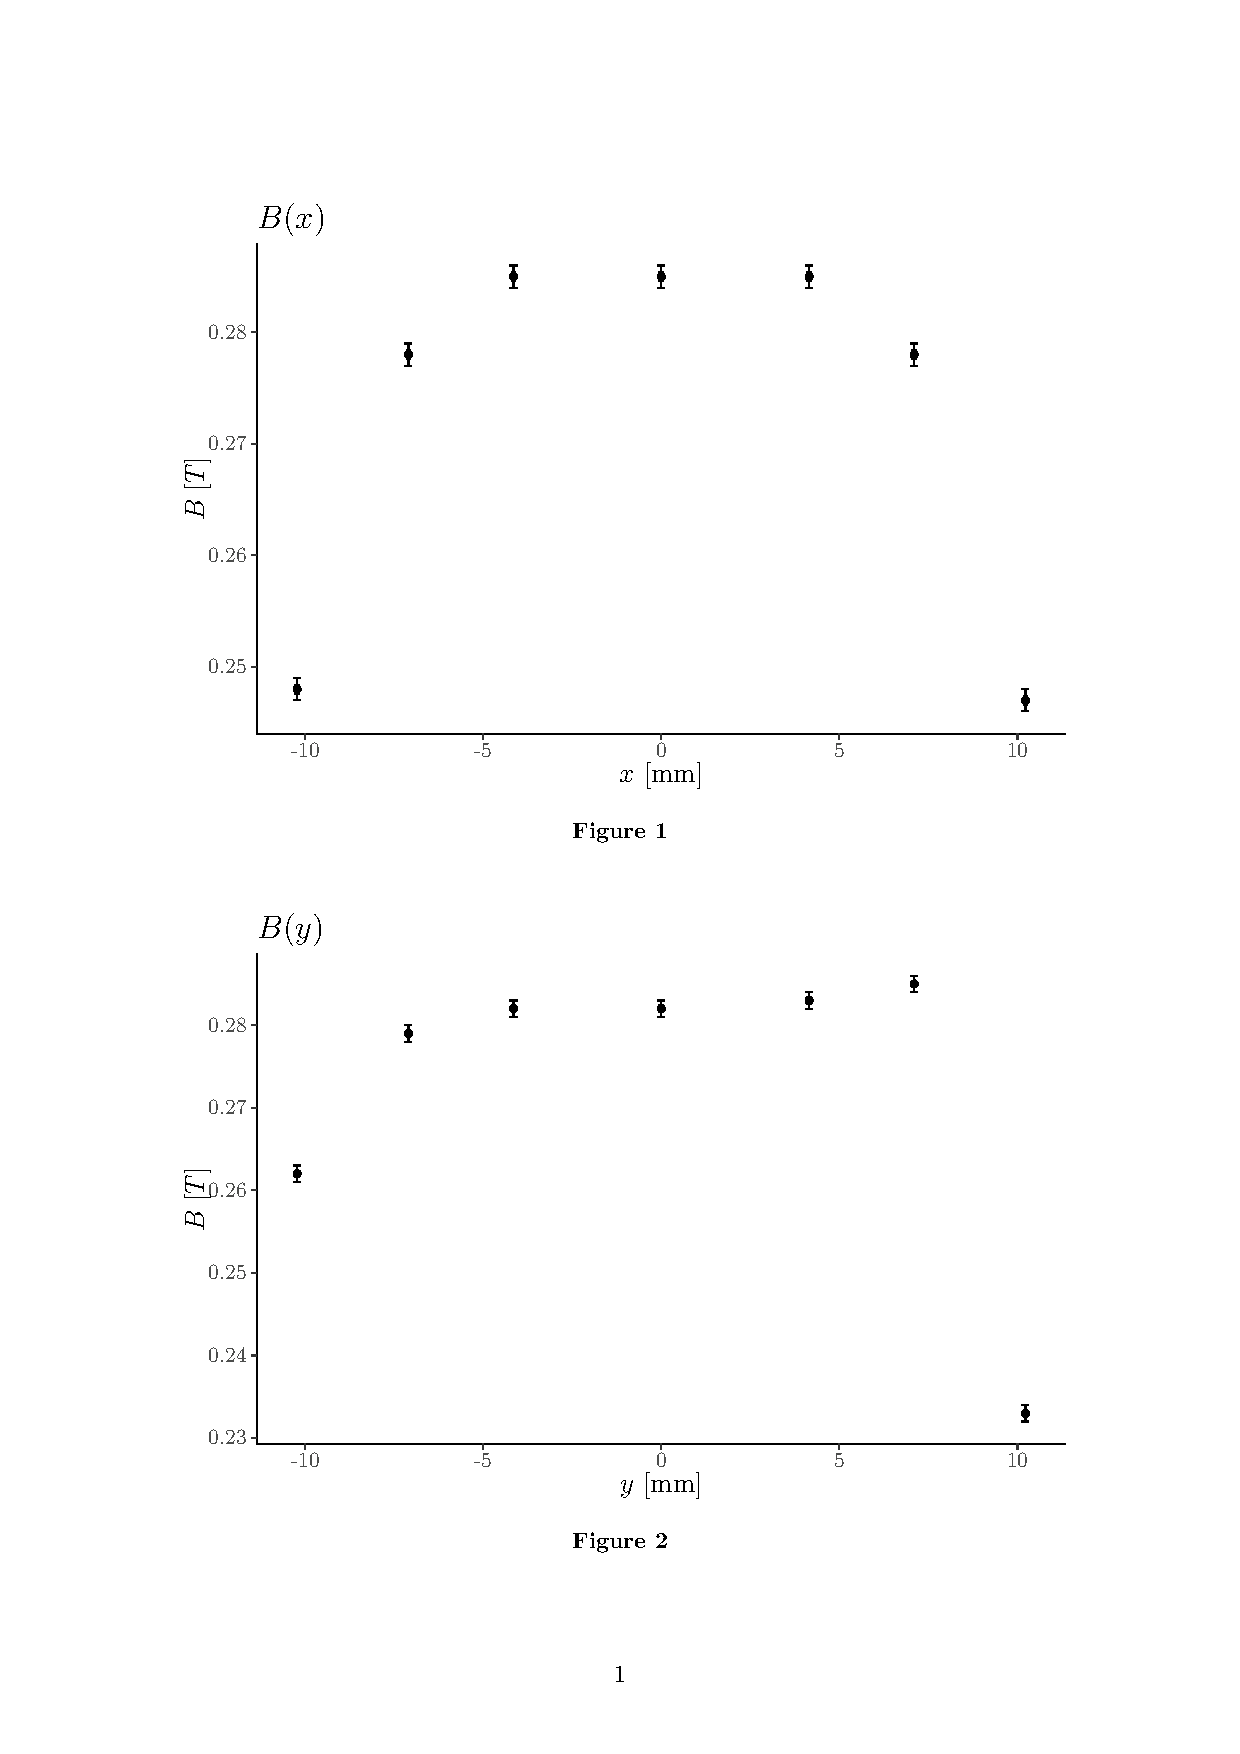
\includegraphics[trim=3cm 16.25cm 3cm 3cm, clip,height=9cm,keepaspectratio]{plots/MagneticDishomogeneity.pdf}
\end{center}
\caption{}
\label{fig:disX}
\end{figure}

\begin{table}[H]
\centering
\caption{}
\label{table:disY}
\resizebox{8cm}{!}{
\begin{tabular}{ccc}
\toprule
$I\;[A]$ & $y$ [mm] & $B\;[T]$       \\
\midrule
\rowcolor{gray!6}  4.13 $\pm$ 0.02 & -10.23 $\pm$ 0.05 & 0.262 $\pm$ 0.001\\
 & -7.10 $\pm$ 0.05  & 0.279 $\pm$ 0.001\\
\rowcolor{gray!6}   & -4.15 $\pm$ 0.05 & 0.282 $\pm$ 0.001\\
 & 0.00 $\pm$ 0.05 & 0.282 $\pm$ 0.001\\
\rowcolor{gray!6}   & 4.15 $\pm$ 0.05 & 0.283 $\pm$ 0.001\\
 & 7.10 $\pm$ 0.05 & 0.285 $\pm$ 0.001\\
\rowcolor{gray!6}   & 10.23 $\pm$ 0.05 & 0.233 $\pm$ 0.001\\
\bottomrule
\end{tabular}}
\end{table}

\begin{figure}[H]
\begin{center}
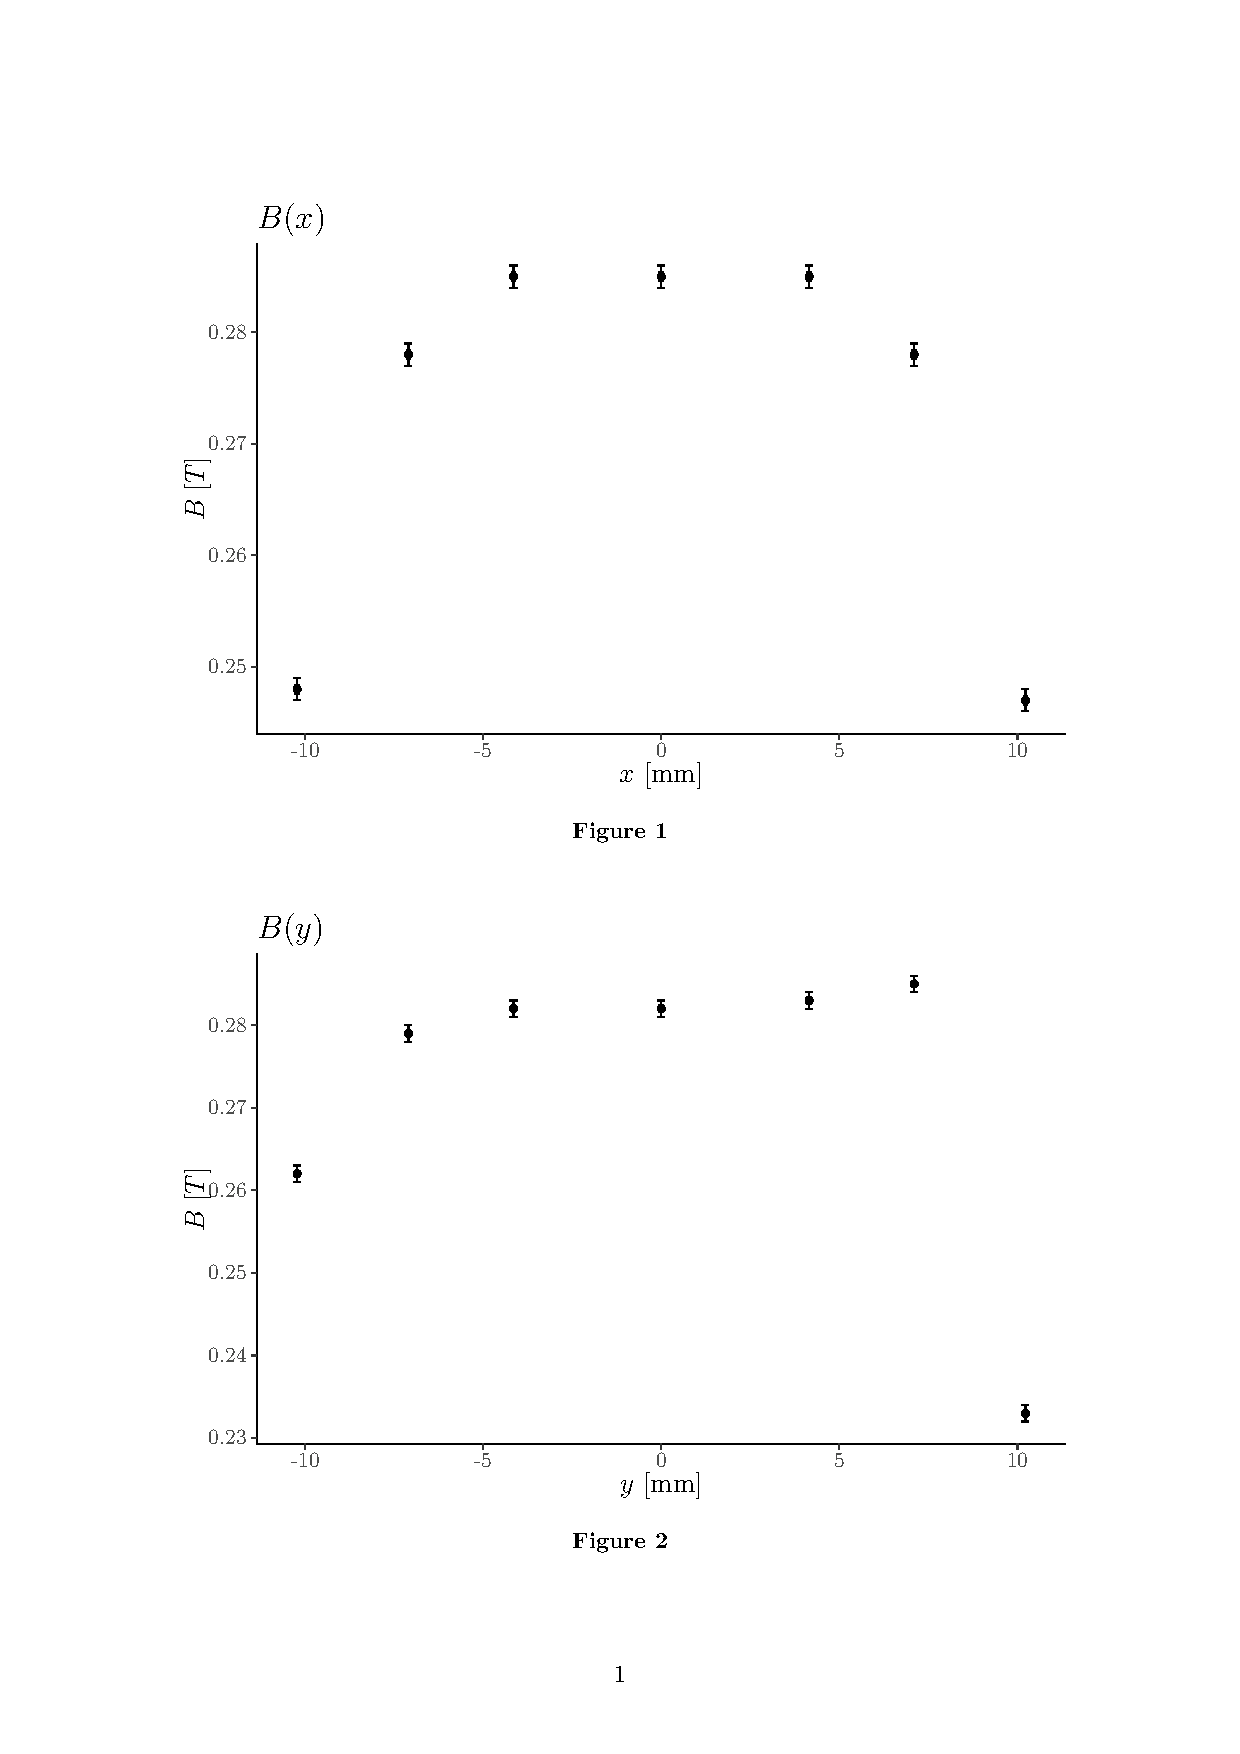
\includegraphics[trim=3cm 4cm 3cm 15cm, clip,height=7cm,keepaspectratio]{plots/MagneticDishomogeneity.pdf}
\end{center}
\caption{}
\label{fig:disY}
\end{figure}

Since the spectroscopic lamp was taller than larger, in order to evaluate the uncertainty of the magnetic field along the $x$ coordinate we have considered only the first four measures around the central position, while to evaluate it along the $y$ coordinate we have considered all the measurements and calculated the maximum semi-dispersions $\Delta_B^x=0.007 \; T$ and $\Delta_B^y=0.052 \; T$ .

Then we have computed the average of the semi-dispersions and the relative error with respect to the maximum value of $B=0.285\;T$, whose results have been reported in \hyperref[table:semi]{ Table \ref*{table:semi}}.

\begin{table}[H]
\centering
\caption{}
\label{table:semi}
\resizebox{8cm}{!}{
\begin{tabular}{cccc}
\toprule
$\Delta_B^x\;[T]$ & $\Delta_B^y\;[T]$ & $\langle \Delta_B \rangle\;[T]$ & $\Delta_{\text{rel}}$       \\
\midrule
\rowcolor{gray!6} 0.007  & 0.052  & 0.0295  & 0.1035087719\\
\bottomrule
\end{tabular}}
\end{table}

From now on the error assigned to the magnetic field will be $\Delta_B=B\Delta_{\text{rel}}$, unless the error propagation derived from the calibration curve yields a larger value. 

\clearpage

\section{Normal Zeeman Effect}

\subsection{Data Collection}

The data regarding the transverse and longitudinal configurations have been collected and reported in \hyperref[table:znt]{Table \ref*{table:znt}} and \hyperref[table:znl]{ \ref*{table:znl}} respectively. The values of $B$ have been derived from those of $I$ in \hyperref[sec:cal]{Calibration Curve}, while $\frac{\langle \delta \rangle}{\langle \Delta \rangle}$ has been calculated as described in \hyperref[sec:ExpIntro]{Experimental Introduction}.

\subsection{Data Analysis \& Visualization}

The datasets concerning the transverse and longitudinal configurations have been fit with the linear model $f(B)=\boldsymbol{p_0}B+\boldsymbol{p_1}$ and plotted in \hyperref[fig:znt]{Figure \ref*{fig:znt}} and \hyperref[fig:znl]{ \ref*{fig:znl}}, together with the respective fit parameters $\boldsymbol{p_0}$ and  $\boldsymbol{p_1}$ .


\begin{table}[H]
\centering
\caption{}
\label{table:znt}
\resizebox{8cm}{!}{
  \begin{tabular}{cccccc}
  \toprule
 $I\;[A]$ & $B\;[T]$ & $\frac{\langle \delta \rangle}{\langle \Delta \rangle}$ \\
  \midrule
  \rowcolor{gray!6}  2.61 $\pm$ 0.02 & 0.183 $\pm$ 0.019 & 0.061 $\pm$ 0.004\\
  4.92 $\pm$ 0.02 & 0.338 $\pm$ 0.035 & 0.125 $\pm$ 0.007\\
  \rowcolor{gray!6}  5.84 $\pm$ 0.02 & 0.400 $\pm$ 0.041 & 0.158 $\pm$ 0.003\\
  6.83 $\pm$ 0.02 & 0.466 $\pm$ 0.048 & 0.188 $\pm$ 0.006\\
  \rowcolor{gray!6}  7.225 $\pm$ 0.025 & 0.500 $\pm$ 0.052 & 0.198 $\pm$ 0.006\\
  7.92 $\pm$ 0.02 & 0.543 $\pm$ 0.056 & 0.221 $\pm$ 0.004\\
  \rowcolor{gray!6}  8.91 $\pm$ 0.02 & 0.596 $\pm$ 0.062 & 0.233 $\pm$ 0.006\\
  9.92 $\pm$ 0.02 & 0.641 $\pm$ 0.066 & 0.263 $\pm$ 0.009\\
  \bottomrule
   \addlinespace
  \end{tabular}}
\end{table}

\begin{figure}[H]
    \centering
    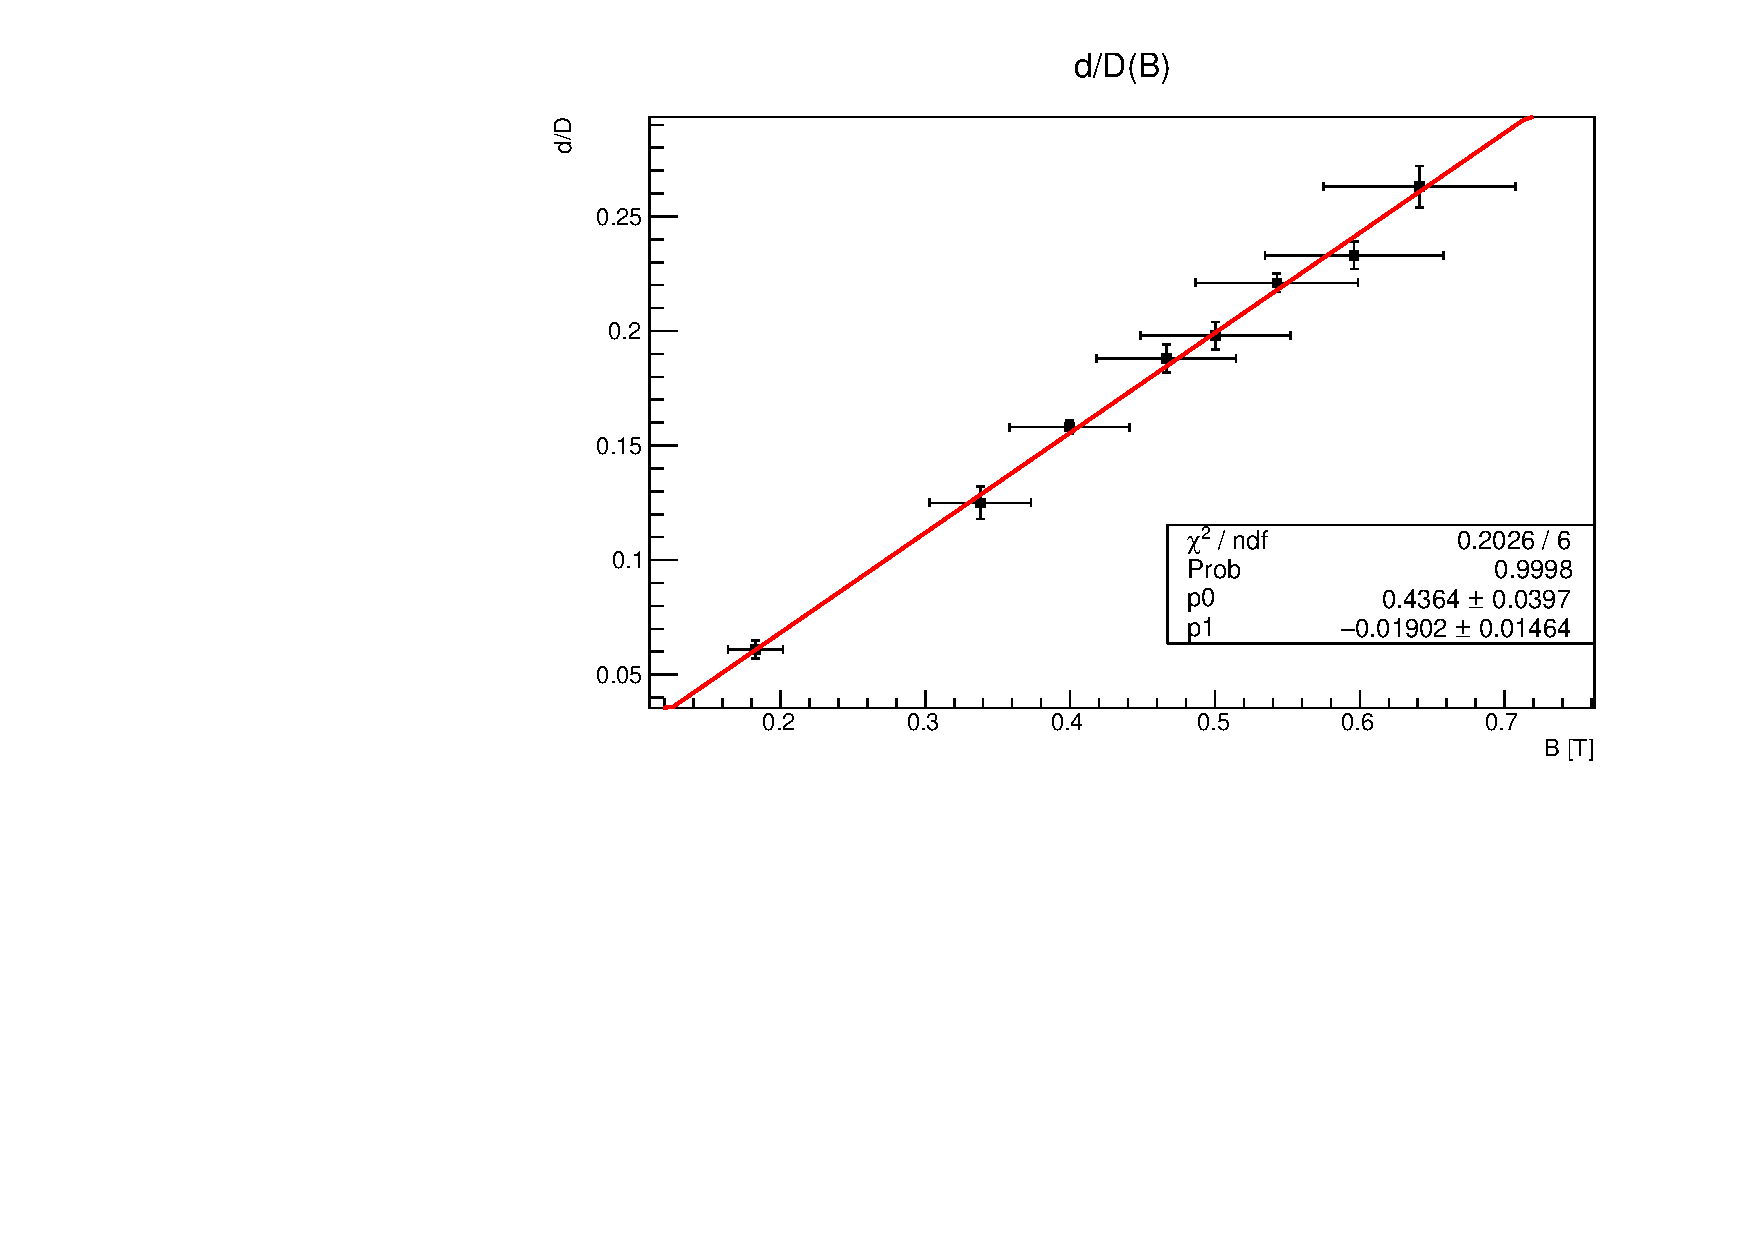
\includegraphics[scale=0.66]{plots/znt.pdf}
    \caption{Transverse}
    \label{fig:znt}
\end{figure}


\begin{table}[H]
\centering
\caption{}
\label{table:znl}
\resizebox{12cm}{!}{
  \begin{tabular}{cccccc}
  \toprule
 $I\;[A]$ & $B\;[T]$ & $\frac{\langle \delta \rangle}{\langle \Delta \rangle}$ \\
  \midrule
  \rowcolor{gray!6}  2.69 $\pm$ 0.02 & 0.188 $\pm$ 0.019 & 0.070 $\pm$ 0.002\\
  4.84 $\pm$ 0.02 & 0.333 $\pm$ 0.034 & 0.140 $\pm$ 0.003\\
  \rowcolor{gray!6}  5.91 $\pm$ 0.02 & 0.404 $\pm$ 0.082 & 0.165 $\pm$ 0.002\\
  6.93 $\pm$ 0.03 & 0.473 $\pm$ 0.049 & 0.192 $\pm$ 0.002\\
  \rowcolor{gray!6}  7.23 $\pm$ 0.02 & 0.500 $\pm$ 0.052 & 0.202 $\pm$ 0.010\\
  7.86 $\pm$ 0.02 & 0.539 $\pm$ 0.056 & 0.218 $\pm$ 0.002\\
  \rowcolor{gray!6}  8.83 $\pm$ 0.02 & 0.592 $\pm$ 0.061 & 0.237 $\pm$ 0.006\\
  9.80 $\pm$ 0.02 & 0.636 $\pm$ 0.066 & 0.263 $\pm$ 0.009\\
  \bottomrule
  \addlinespace
    \addlinespace
  \addlinespace
  \addlinespace
  \addlinespace
  \addlinespace
  \addlinespace
   \addlinespace
  \end{tabular}}
\end{table}

\begin{figure}[H]
    \centering
    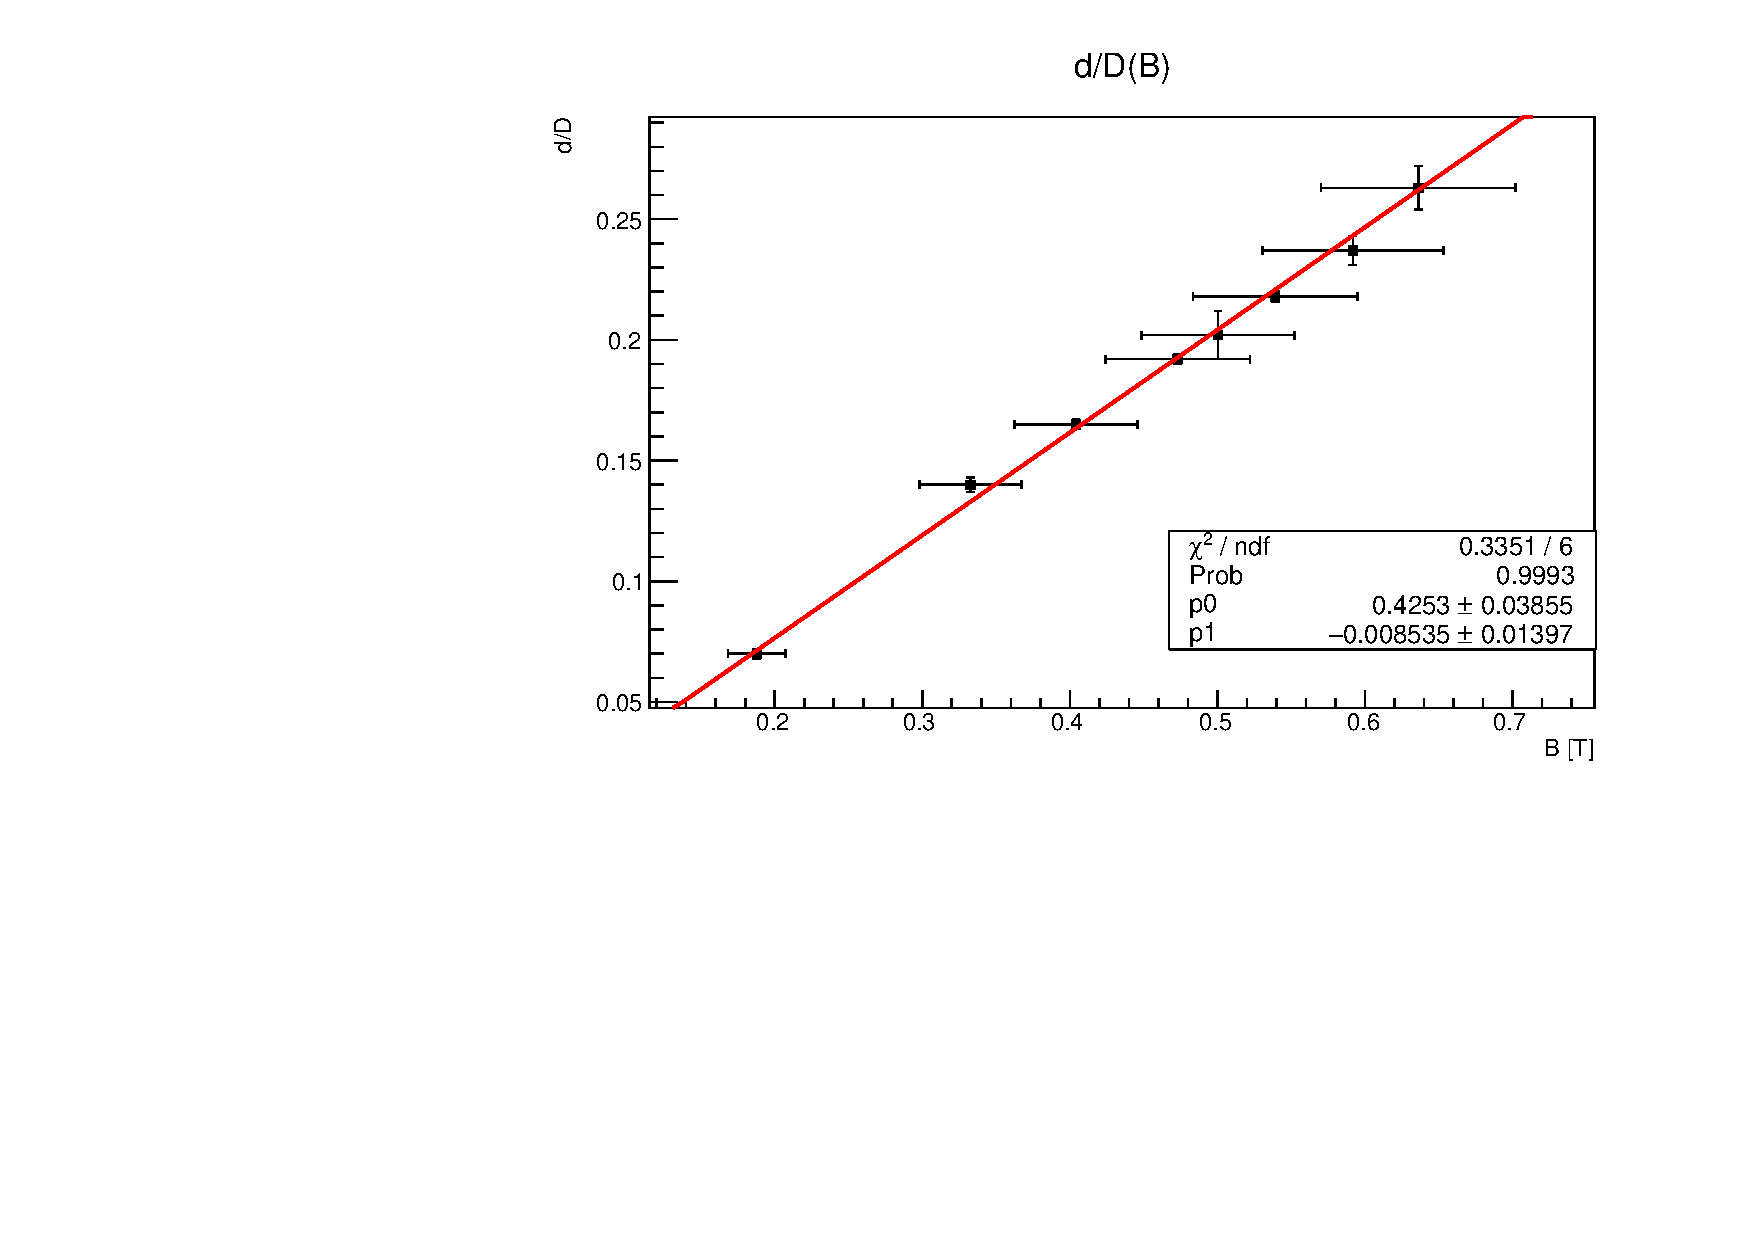
\includegraphics[scale=0.85]{plots/znl.pdf}
    \caption{Longitudinal}
    \label{fig:znl}
\end{figure}
        
\clearpage

\subsection{Bohr Magneton}
Now it is possible to calculate the Bohr magneton for both configurations $$\mu_N^T= (\boldsymbol{p_0^T}\pm \boldsymbol{\delta p_0^T})\frac{hc}{2g_n\mu_n w} \quad\text{and}\quad \mu_N^L= (\boldsymbol{p_0^L}\pm \boldsymbol{\delta p_0^L})\frac{hc}{2g_n\mu_n w}$$ 
 since we know 
\begin{itemize}
\item $h=6.626070040\times10^{-34} \text{ Js}  \;\,\quad\qquad\qquad\text{ Plack constant}$  
\item $c=299792458 \text{ ms}^{-1}  \quad\qquad\qquad\qquad\qquad\text{speed of light in the vacuum}$
\item $g_n=1   \;\;\qquad\qquad\qquad\qquad\qquad\qquad\qquad\text{ gyromagnetic factor}$
\item $\mu_n= 1.4560    \;\qquad\qquad\qquad\qquad\qquad\qquad\text{ refractive index}$
\item  $w= 0.003 \text{ m} \;\qquad\qquad\qquad\qquad\qquad\qquad\text{thickness}$
\item $\boldsymbol{p_0^{T}}=0.436 \pm 0.040 \;\text{T}^{-1} \;\quad\qquad\qquad\qquad\text{ transverse slope}$
\item $\boldsymbol{p_0^{L}}=0.425 \pm 0.039 \;\text{T}^{-1} \;\quad\qquad\qquad\qquad\text{ longitudinal slope .}$\newline
\end{itemize}
The compatibility between $\mu_N^T$ and $\mu_N^L$ has been tested as displayed in \hyperref[table:Zn]{Table \ref*{table:Zn}}. 
\begin{table}[H]
\caption{}
\centering
\resizebox{10cm}{!}{
\begin{tabular}{cccc}
\toprule
$\mu_N^T\;[\text{JT}^{-1}]$ & $\mu_N^L\;[\text{JT}^{-1}]$ & $Z$ & Compatibility  \\
\midrule
\rowcolor{gray!6} $9.91 \pm  0.91\times 10^{-24}$ & $9.66 \pm  0.89\times 10^{-24}$ & 0.20 & \checkmark \\
\bottomrule
\end{tabular}}
\label{table:Zn}
\end{table}

Since the result has been positive, we have calculated the weighted average $ \langle \mu_N\rangle$ and tested against the theoretical value $\boldsymbol{\mu_B}$ as shown in \hyperref[table:ZnT]{Table \ref*{table:ZnT}} .

\begin{table}[H]
\caption{}
\centering
\resizebox{10cm}{!}{
\begin{tabular}{cccc}
\toprule
$\langle \mu_N \rangle \;[\text{JT}^{-1}]$ & $\boldsymbol{\mu_B} \;[\text{JT}^{-1}]$ & $Z$ & Compatibility  \\
\midrule
\rowcolor{gray!6} $9.79 \pm 0.63 \times 10^{-24}$ & $9.27 \times 10^{-24}$ & 0.41 & \checkmark \\
\bottomrule
\end{tabular}}
\label{table:ZnT}
\end{table}

\clearpage

\section{Anomalous Zeeman Effect}

\subsection{Data Collection}

The data regarding the transverse and longitudinal configurations have been collected and reported in \hyperref[table:zat]{Table \ref*{table:zat}} and \hyperref[table:zal]{ \ref*{table:zal}} respectively. The values of $B$ have been derived from those of $I$ in \hyperref[sec:cal]{Calibration Curve}, while $\frac{\langle \delta \rangle}{\langle \Delta \rangle}$ has been calculated as described in \hyperref[sec:ExpIntro]{Experimental Introduction}.

\subsection{Data Analysis \& Visualization}

The datasets concerning the transverse and longitudinal configurations have been fit with the linear model $f(B)=\boldsymbol{p_0}B+\boldsymbol{p_1}$ and plotted in \hyperref[fig:zat]{Figure \ref*{fig:zat}} and \hyperref[fig:zal]{ \ref*{fig:zal}}, together with the respective fit parameters $\boldsymbol{p_0}$ and  $\boldsymbol{p_1}$ .


\begin{table}[H]
\centering
\caption{}
\label{table:zat}
\resizebox{8.2cm}{!}{
  \begin{tabular}{cccccc}
  \toprule
 $I\;[A]$ & $B\;[T]$ & $\frac{\langle \delta \rangle}{\langle \Delta \rangle}$ \\
  \midrule
  \rowcolor{gray!6}  5.75 $\pm$ 0.04 & 0.394 $\pm$ 0.041 & 0.062 $\pm$ 0.002\\
  6.74 $\pm$ 0.02 & 0.460 $\pm$ 0.048 & 0.081 $\pm$ 0.021\\
  \rowcolor{gray!6}  7.275 $\pm$ 0.025 & 0.504 $\pm$ 0.052 & 0.098 $\pm$ 0.019\\
  7.82 $\pm$ 0.02 & 0.537 $\pm$ 0.056 & 0.086 $\pm$ 0.034\\
  \rowcolor{gray!6}  8.795 $\pm$ 0.095 & 0.590 $\pm$ 0.061 & 0.096 $\pm$ 0.030\\
  9.95 $\pm$ 0.04 & 0.642 $\pm$ 0.066 & 0.082 $\pm$ 0.032\\
  \bottomrule
  \end{tabular}}
\end{table}

\begin{figure}[H]
     \centering
     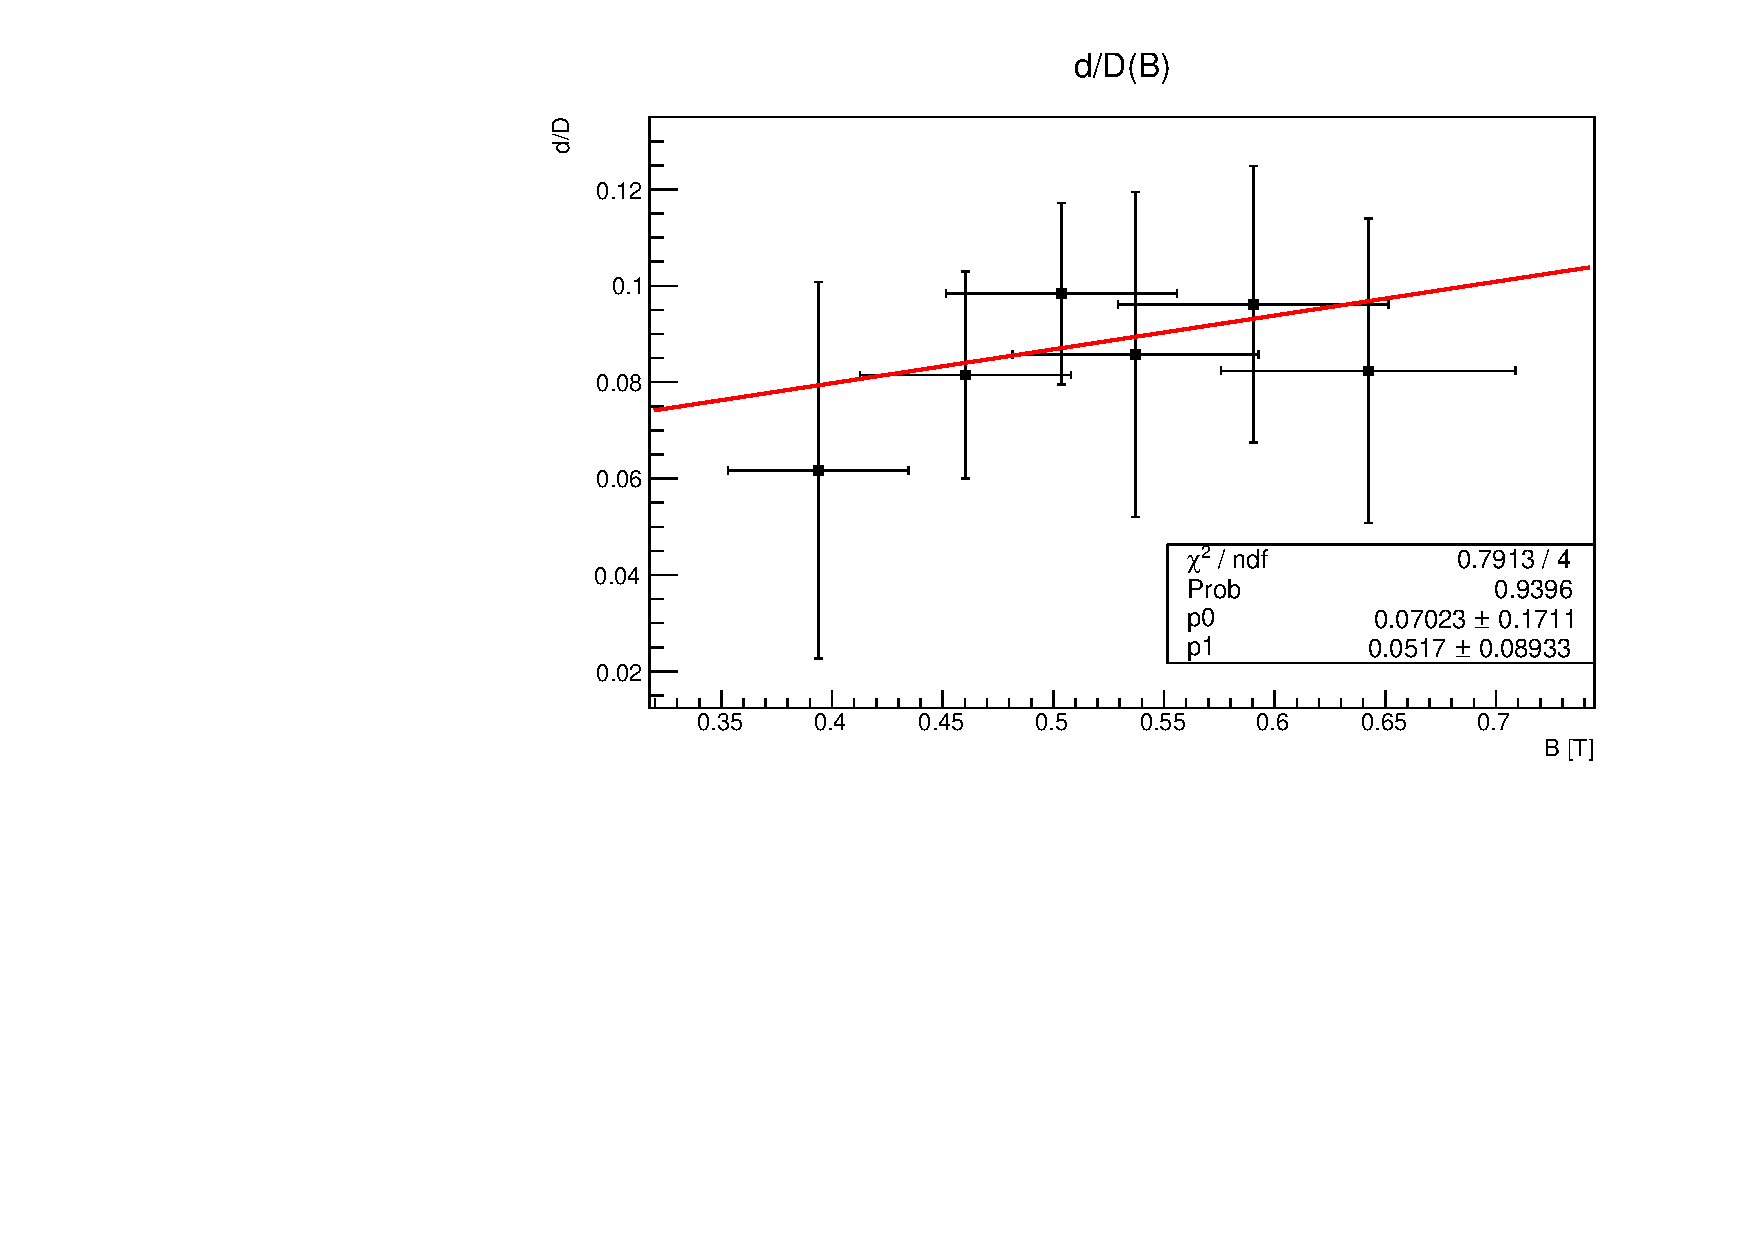
\includegraphics[scale=0.76]{plots/zat.pdf}
    \caption{Transverse}
    \label{fig:zat}
\end{figure}

\begin{table}[H]
\centering
\caption{}
\label{table:zal}
\resizebox{12cm}{!}{
  \begin{tabular}{cccccc}
  \toprule
 $I\;[A]$ & $B\;[T]$ & $\frac{\langle \delta \rangle}{\langle \Delta \rangle}$ \\
  \midrule
  \rowcolor{gray!6}  7.31 $\pm$ 0.02 & 0.506 $\pm$ 0.052 & 0.057 $\pm$ 0.011\\
  7.85 $\pm$ 0.02 & 0.539 $\pm$ 0.056 & 0.069 $\pm$ 0.012\\
  \rowcolor{gray!6}  8.32 $\pm$ 0.02 & 0.565 $\pm$ 0.059 & 0.088 $\pm$ 0.017\\
  8.84 $\pm$ 0.02 & 0.593 $\pm$ 0.061 & 0.128 $\pm$ 0.031\\
  \rowcolor{gray!6}  9.415 $\pm$ 0.025 & 0.620 $\pm$ 0.064 & 0.147 $\pm$ 0.022\\
  9.99 $\pm$ 0.02 & 0.644 $\pm$ 0.067 & 0.130 $\pm$ 0.022\\
  \bottomrule
  \addlinespace
    \addlinespace
  \addlinespace
  \addlinespace
  \addlinespace
  \end{tabular}}
\end{table}
\begin{figure}[H]
   \hspace{-1.7cm} 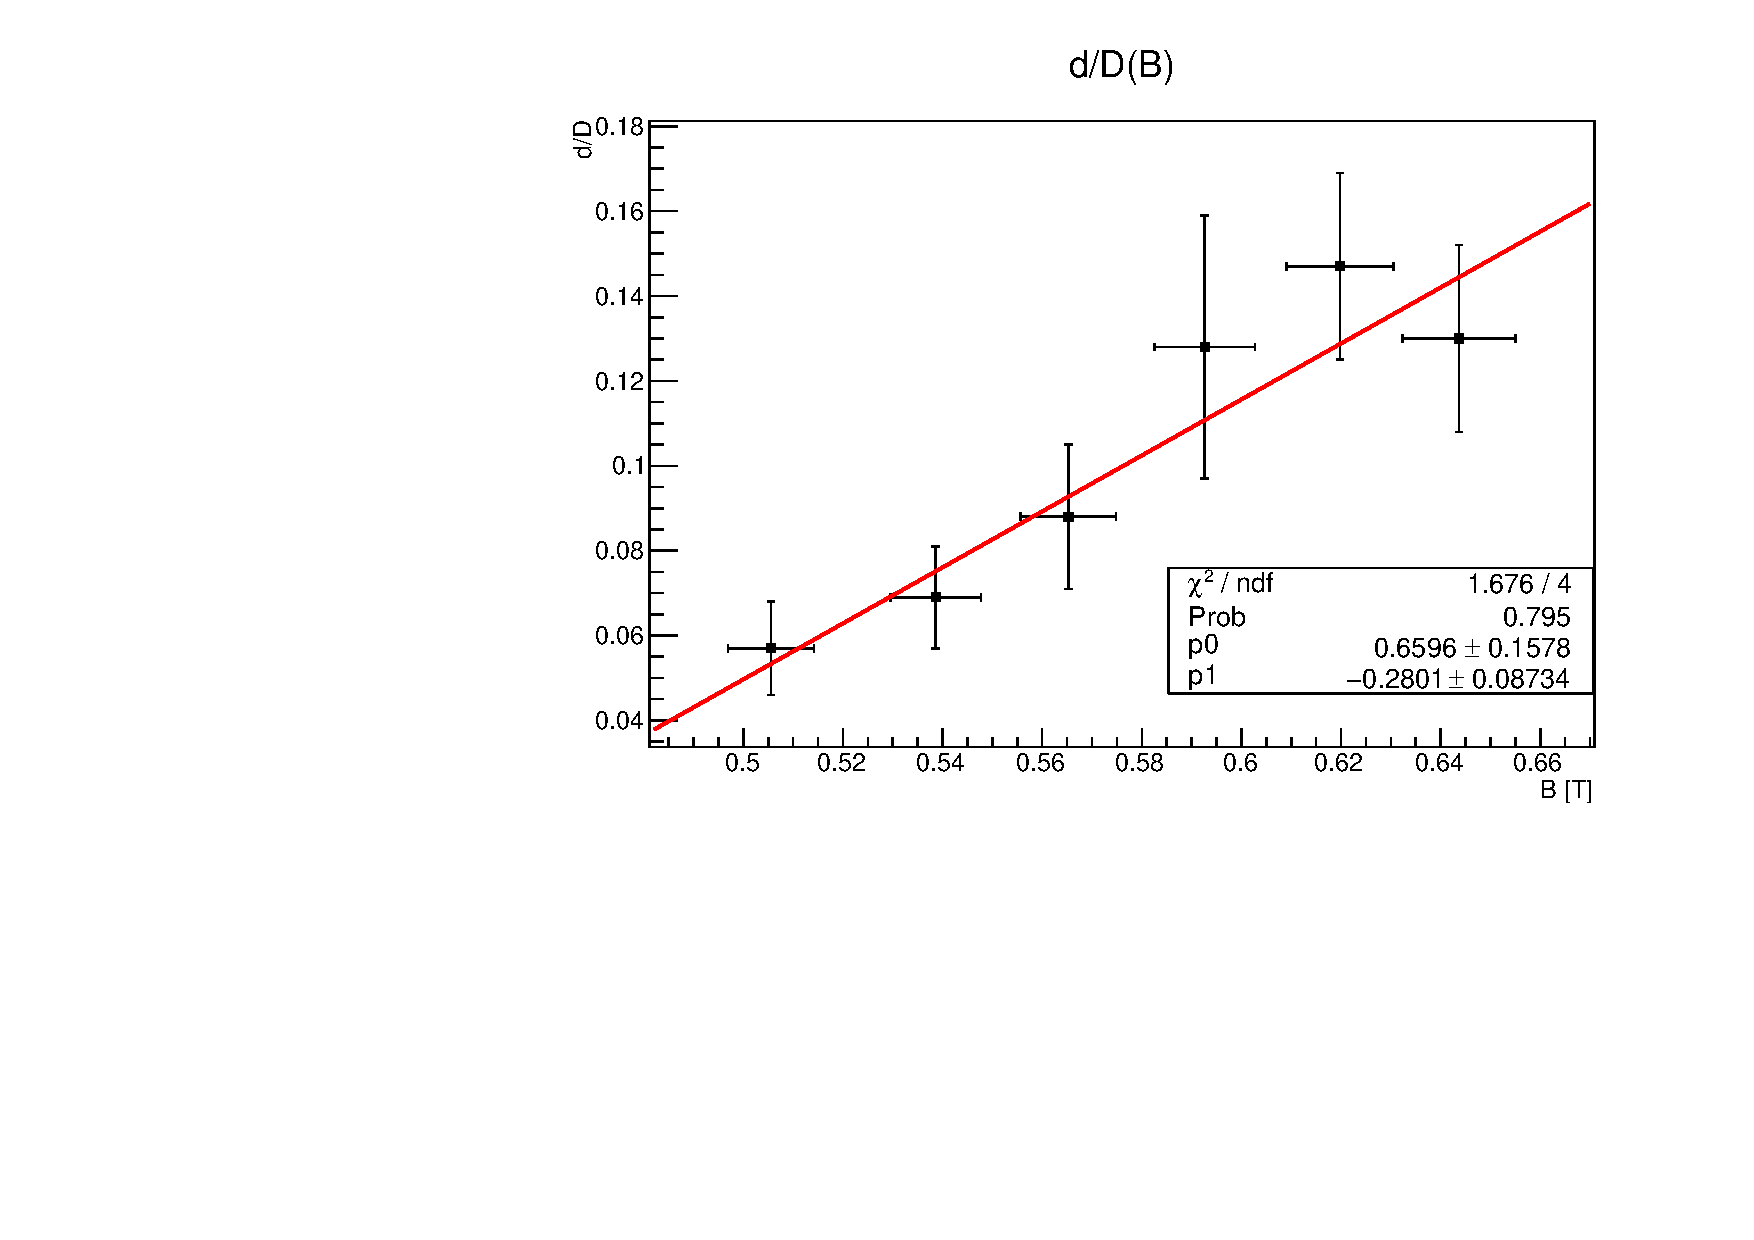
\includegraphics[scale=0.95]{plots/zal.pdf}
    \caption{Longitudinal}
    \label{fig:zal}
\end{figure}

\subsection{Bohr Magneton}
Now it is possible to calculate the Bohr magneton for both configurations $$\mu_A^T= (\boldsymbol{p_0^T}\pm \boldsymbol{\delta p_0^T})\frac{hc}{2g_a\mu_a w} \quad\text{and}\quad \mu_A^L= (\boldsymbol{p_0^L}\pm \boldsymbol{\delta p_0^L})\frac{hc}{2g_a\mu_a w}$$ 
 since we know 
\begin{itemize}
\item $h=6.626070040\times10^{-34} \text{ Js}  \;\,\quad\qquad\qquad\text{ Plack constant}$  
\item $c=299792458 \text{ ms}^{-1}  \quad\qquad\qquad\qquad\qquad\text{speed of light in the vacuum}$
\item $g_a=1/2   \;\;\quad\qquad\qquad\qquad\qquad\qquad\qquad\text{ gyromagnetic factor}$
\item $\mu_a= 1.4560    \;\qquad\qquad\qquad\qquad\qquad\qquad\text{ refractive index}$
\item  $w= 0.003 \text{ m} \;\qquad\qquad\qquad\qquad\qquad\qquad\text{thickness}$
\item $\boldsymbol{p_0^{T}}=0.070 \pm 0.171 \;\text{T}^{-1}
\;\quad\qquad\qquad\qquad\text{ transverse slope}$
\item $\boldsymbol{p_0^{L}}=0.737 \pm 0.433 \;\text{T}^{-1} \;\quad\qquad\qquad\qquad\text{ longitudinal slope .}$\newline
\end{itemize} 

The compatibility between $\mu_A^T$ and $\mu_A^L$ has been tested as displayed in \hyperref[table:Za]{Table \ref*{table:Za}}. 
\begin{table}[H]
\caption{}
\centering
\resizebox{11cm}{!}{
\begin{tabular}{cccc}
\toprule
$\mu_A^T\;[\text{JT}^{-1}]$ & $\mu_A^L\;[\text{JT}^{-1}]$ & $Z$ & Compatibility  \\
\midrule
\rowcolor{gray!6} $3.20 \pm 7.80\times 10^{-24}$ & $33.61 \pm 19.75$ & 1.43 & \checkmark \\
\bottomrule
\end{tabular}}
\label{table:Za}
\end{table}

Since the result has been positive, we have calculated the weighted average $$ \langle \mu_A\rangle=7.30 \pm 7.25\times 10^{-24}\;\text{JT}^{-1}\;.$$

% footnote ZN VS ZA : due to experimental limits (see notes) and expected complications 

Then the compatibility test between $\langle \mu_A \rangle$ and $\langle \mu_N \rangle$ has been computed and displayed in \hyperref[table:Zan]{Table \ref*{table:Zan}}. 
\begin{table}[H]
\caption{}
\centering
\resizebox{11cm}{!}{
\begin{tabular}{cccc}
\toprule
$\langle \mu_A \rangle\;[\text{JT}^{-1}]$ & $\langle \mu_N \rangle\;[\text{JT}^{-1}]$ & $Z$ & Compatibility  \\
\midrule
\rowcolor{gray!6} $7.30 \pm 7.25\times 10^{-24}$ & $9.79 \pm 6.63$ & 0.34 & \checkmark \\
\bottomrule
\end{tabular}}
\label{table:Zan}
\end{table}

Since the result has been positive, we have calculated the global weighted average $$ \langle \mu\rangle=9.77 \pm  0.63\times 10^{-24}\;\text{JT}^{-1}$$ which has been tested against the theoretical value $\boldsymbol{\mu_B}$ as shown in \hyperref[table:Z]{Table \ref*{table:Z}} .

\begin{table}[H]
\caption{}
\centering
\resizebox{11cm}{!}{
\begin{tabular}{cccc}
\toprule
$\langle \mu \rangle \;[\text{JT}^{-1}]$ & $\boldsymbol{\mu_B} \;[\text{JT}^{-1}]$ & $Z$ & Compatibility  \\
\midrule
\rowcolor{gray!6} $9.77 \pm  0.63 \times 10^{-24}$ & $9.27 \times 10^{-24}$ & 0.79 & \checkmark \\
\bottomrule
\end{tabular}}
\label{table:Z}
\end{table}


\subsubsection{Alternative Method}
 \subsubsection{Approximation Methods}
1. Observations of previous results 
2. System of co-causes : 
   2.1 Experimental limitations --> reduced resolutions of CCD --> indistinguishibility --> perceived width >> normal case --> Superpositions of light signals associated with different orders
   2.2 Low accuracy of $\Delta r /2$ methods (image comparison) 
   2.3 Large error on B due to \ref{sec: MagHom} 

   HOMOGENEOUS TRIGONOMETRIC METHOD 


\clearpage


\section{Conclusions}

\section{Appendix}

%\bibliographystyle{unsrt}
%\bibliography{biblio}
\end{document}
